\documentclass[twoside]{book}

% Packages required by doxygen
\usepackage{fixltx2e}
\usepackage{calc}
\usepackage{doxygen}
\usepackage[export]{adjustbox} % also loads graphicx
\usepackage{graphicx}
\usepackage[utf8]{inputenc}
\usepackage{makeidx}
\usepackage{multicol}
\usepackage{multirow}
\PassOptionsToPackage{warn}{textcomp}
\usepackage{textcomp}
\usepackage[nointegrals]{wasysym}
\usepackage[table]{xcolor}

% Font selection
\usepackage[T1]{fontenc}
\usepackage[scaled=.90]{helvet}
\usepackage{courier}
\usepackage{amssymb}
\usepackage{sectsty}
\renewcommand{\familydefault}{\sfdefault}
\allsectionsfont{%
  \fontseries{bc}\selectfont%
  \color{darkgray}%
}
\renewcommand{\DoxyLabelFont}{%
  \fontseries{bc}\selectfont%
  \color{darkgray}%
}
\newcommand{\+}{\discretionary{\mbox{\scriptsize$\hookleftarrow$}}{}{}}

% Page & text layout
\usepackage{geometry}
\geometry{%
  a4paper,%
  top=2.5cm,%
  bottom=2.5cm,%
  left=2.5cm,%
  right=2.5cm%
}
\tolerance=750
\hfuzz=15pt
\hbadness=750
\setlength{\emergencystretch}{15pt}
\setlength{\parindent}{0cm}
\setlength{\parskip}{3ex plus 2ex minus 2ex}
\makeatletter
\renewcommand{\paragraph}{%
  \@startsection{paragraph}{4}{0ex}{-1.0ex}{1.0ex}{%
    \normalfont\normalsize\bfseries\SS@parafont%
  }%
}
\renewcommand{\subparagraph}{%
  \@startsection{subparagraph}{5}{0ex}{-1.0ex}{1.0ex}{%
    \normalfont\normalsize\bfseries\SS@subparafont%
  }%
}
\makeatother

% Headers & footers
\usepackage{fancyhdr}
\pagestyle{fancyplain}
\fancyhead[LE]{\fancyplain{}{\bfseries\thepage}}
\fancyhead[CE]{\fancyplain{}{}}
\fancyhead[RE]{\fancyplain{}{\bfseries\leftmark}}
\fancyhead[LO]{\fancyplain{}{\bfseries\rightmark}}
\fancyhead[CO]{\fancyplain{}{}}
\fancyhead[RO]{\fancyplain{}{\bfseries\thepage}}
\fancyfoot[LE]{\fancyplain{}{}}
\fancyfoot[CE]{\fancyplain{}{}}
\fancyfoot[RE]{\fancyplain{}{\bfseries\scriptsize Generated by Doxygen }}
\fancyfoot[LO]{\fancyplain{}{\bfseries\scriptsize Generated by Doxygen }}
\fancyfoot[CO]{\fancyplain{}{}}
\fancyfoot[RO]{\fancyplain{}{}}
\renewcommand{\footrulewidth}{0.4pt}
\renewcommand{\chaptermark}[1]{%
  \markboth{#1}{}%
}
\renewcommand{\sectionmark}[1]{%
  \markright{\thesection\ #1}%
}

% Indices & bibliography
\usepackage{natbib}
\usepackage[titles]{tocloft}
\setcounter{tocdepth}{3}
\setcounter{secnumdepth}{5}
\makeindex

% Hyperlinks (required, but should be loaded last)
\usepackage{ifpdf}
\ifpdf
  \usepackage[pdftex,pagebackref=true]{hyperref}
\else
  \usepackage[ps2pdf,pagebackref=true]{hyperref}
\fi
\hypersetup{%
  colorlinks=true,%
  linkcolor=blue,%
  citecolor=blue,%
  unicode%
}

% Custom commands
\newcommand{\clearemptydoublepage}{%
  \newpage{\pagestyle{empty}\cleardoublepage}%
}

\usepackage{caption}
\captionsetup{labelsep=space,justification=centering,font={bf},singlelinecheck=off,skip=4pt,position=top}

%===== C O N T E N T S =====

\begin{document}

% Titlepage & ToC
\hypersetup{pageanchor=false,
             bookmarksnumbered=true,
             pdfencoding=unicode
            }
\pagenumbering{alph}
\begin{titlepage}
\vspace*{7cm}
\begin{center}%
{\Large My Project }\\
\vspace*{1cm}
{\large Generated by Doxygen 1.8.12}\\
\end{center}
\end{titlepage}
\clearemptydoublepage
\pagenumbering{roman}
\tableofcontents
\clearemptydoublepage
\pagenumbering{arabic}
\hypersetup{pageanchor=true}

%--- Begin generated contents ---
\chapter{Hierarchical Index}
\section{Class Hierarchy}
This inheritance list is sorted roughly, but not completely, alphabetically\+:\begin{DoxyCompactList}
\item \contentsline{section}{org.\+jcs.\+dss.\+op.\+Object\+To\+X\+ML}{\pageref{classorg_1_1jcs_1_1dss_1_1op_1_1ObjectToXML}}{}
\item \contentsline{section}{org.\+jcs.\+dss.\+op.\+Op}{\pageref{classorg_1_1jcs_1_1dss_1_1op_1_1Op}}{}
\begin{DoxyCompactList}
\item \contentsline{section}{org.\+jcs.\+dss.\+op.\+Bucket\+Op}{\pageref{classorg_1_1jcs_1_1dss_1_1op_1_1BucketOp}}{}
\begin{DoxyCompactList}
\item \contentsline{section}{org.\+jcs.\+dss.\+op.\+Create\+Bucket\+Op}{\pageref{classorg_1_1jcs_1_1dss_1_1op_1_1CreateBucketOp}}{}
\item \contentsline{section}{org.\+jcs.\+dss.\+op.\+Delete\+Bucket\+Op}{\pageref{classorg_1_1jcs_1_1dss_1_1op_1_1DeleteBucketOp}}{}
\item \contentsline{section}{org.\+jcs.\+dss.\+op.\+Head\+Bucket\+Op}{\pageref{classorg_1_1jcs_1_1dss_1_1op_1_1HeadBucketOp}}{}
\item \contentsline{section}{org.\+jcs.\+dss.\+op.\+List\+Buckets\+Op}{\pageref{classorg_1_1jcs_1_1dss_1_1op_1_1ListBucketsOp}}{}
\item \contentsline{section}{org.\+jcs.\+dss.\+op.\+List\+M\+P\+Uploads\+Op}{\pageref{classorg_1_1jcs_1_1dss_1_1op_1_1ListMPUploadsOp}}{}
\item \contentsline{section}{org.\+jcs.\+dss.\+op.\+List\+Objects\+Op}{\pageref{classorg_1_1jcs_1_1dss_1_1op_1_1ListObjectsOp}}{}
\end{DoxyCompactList}
\item \contentsline{section}{org.\+jcs.\+dss.\+op.\+Object\+Op}{\pageref{classorg_1_1jcs_1_1dss_1_1op_1_1ObjectOp}}{}
\begin{DoxyCompactList}
\item \contentsline{section}{org.\+jcs.\+dss.\+op.\+Cancel\+M\+P\+Upload\+Op}{\pageref{classorg_1_1jcs_1_1dss_1_1op_1_1CancelMPUploadOp}}{}
\item \contentsline{section}{org.\+jcs.\+dss.\+op.\+Complete\+M\+P\+Upload\+Op}{\pageref{classorg_1_1jcs_1_1dss_1_1op_1_1CompleteMPUploadOp}}{}
\item \contentsline{section}{org.\+jcs.\+dss.\+op.\+Copy\+Object\+Op}{\pageref{classorg_1_1jcs_1_1dss_1_1op_1_1CopyObjectOp}}{}
\item \contentsline{section}{org.\+jcs.\+dss.\+op.\+Delete\+Object\+Op}{\pageref{classorg_1_1jcs_1_1dss_1_1op_1_1DeleteObjectOp}}{}
\item \contentsline{section}{org.\+jcs.\+dss.\+op.\+Get\+Object\+Detail\+Op}{\pageref{classorg_1_1jcs_1_1dss_1_1op_1_1GetObjectDetailOp}}{}
\item \contentsline{section}{org.\+jcs.\+dss.\+op.\+Get\+Object\+Op}{\pageref{classorg_1_1jcs_1_1dss_1_1op_1_1GetObjectOp}}{}
\item \contentsline{section}{org.\+jcs.\+dss.\+op.\+Get\+Presigned\+U\+R\+L\+Op}{\pageref{classorg_1_1jcs_1_1dss_1_1op_1_1GetPresignedURLOp}}{}
\item \contentsline{section}{org.\+jcs.\+dss.\+op.\+Head\+Object\+Op}{\pageref{classorg_1_1jcs_1_1dss_1_1op_1_1HeadObjectOp}}{}
\item \contentsline{section}{org.\+jcs.\+dss.\+op.\+Init\+M\+P\+Upload\+Op}{\pageref{classorg_1_1jcs_1_1dss_1_1op_1_1InitMPUploadOp}}{}
\item \contentsline{section}{org.\+jcs.\+dss.\+op.\+List\+Part\+Op}{\pageref{classorg_1_1jcs_1_1dss_1_1op_1_1ListPartOp}}{}
\item \contentsline{section}{org.\+jcs.\+dss.\+op.\+Put\+Object\+Op}{\pageref{classorg_1_1jcs_1_1dss_1_1op_1_1PutObjectOp}}{}
\item \contentsline{section}{org.\+jcs.\+dss.\+op.\+Upload\+Part\+Op}{\pageref{classorg_1_1jcs_1_1dss_1_1op_1_1UploadPartOp}}{}
\end{DoxyCompactList}
\end{DoxyCompactList}
\item \contentsline{section}{org.\+jcs.\+dss.\+op.\+Part\+Creation\+For\+Upload\+Part}{\pageref{classorg_1_1jcs_1_1dss_1_1op_1_1PartCreationForUploadPart}}{}
\end{DoxyCompactList}

\chapter{Class Index}
\section{Class List}
Here are the classes, structs, unions and interfaces with brief descriptions\+:\begin{DoxyCompactList}
\item\contentsline{section}{\hyperlink{classorg_1_1jcs_1_1dss_1_1op_1_1BucketOp}{org.\+jcs.\+dss.\+op.\+Bucket\+Op} \\*Head Class for all operations related to bucket }{\pageref{classorg_1_1jcs_1_1dss_1_1op_1_1BucketOp}}{}
\item\contentsline{section}{\hyperlink{classorg_1_1jcs_1_1dss_1_1op_1_1CancelMPUploadOp}{org.\+jcs.\+dss.\+op.\+Cancel\+M\+P\+Upload\+Op} \\*Sets constructors like http\+Method, query\+String, etc to Cancel a multipart upload }{\pageref{classorg_1_1jcs_1_1dss_1_1op_1_1CancelMPUploadOp}}{}
\item\contentsline{section}{\hyperlink{classorg_1_1jcs_1_1dss_1_1op_1_1CompleteMPUploadOp}{org.\+jcs.\+dss.\+op.\+Complete\+M\+P\+Upload\+Op} \\*Class to execute Complete multipart upload }{\pageref{classorg_1_1jcs_1_1dss_1_1op_1_1CompleteMPUploadOp}}{}
\item\contentsline{section}{\hyperlink{classorg_1_1jcs_1_1dss_1_1op_1_1CopyObjectOp}{org.\+jcs.\+dss.\+op.\+Copy\+Object\+Op} \\*Class to execute method for copying Object from one bucket to another }{\pageref{classorg_1_1jcs_1_1dss_1_1op_1_1CopyObjectOp}}{}
\item\contentsline{section}{\hyperlink{classorg_1_1jcs_1_1dss_1_1op_1_1CreateBucketOp}{org.\+jcs.\+dss.\+op.\+Create\+Bucket\+Op} \\*Class to create a new bucket }{\pageref{classorg_1_1jcs_1_1dss_1_1op_1_1CreateBucketOp}}{}
\item\contentsline{section}{\hyperlink{classorg_1_1jcs_1_1dss_1_1op_1_1DeleteBucketOp}{org.\+jcs.\+dss.\+op.\+Delete\+Bucket\+Op} \\*Class to Delete an existing bucket }{\pageref{classorg_1_1jcs_1_1dss_1_1op_1_1DeleteBucketOp}}{}
\item\contentsline{section}{\hyperlink{classorg_1_1jcs_1_1dss_1_1op_1_1DeleteObjectOp}{org.\+jcs.\+dss.\+op.\+Delete\+Object\+Op} \\*Class to Delete an existing key inside the requested bucket }{\pageref{classorg_1_1jcs_1_1dss_1_1op_1_1DeleteObjectOp}}{}
\item\contentsline{section}{\hyperlink{classorg_1_1jcs_1_1dss_1_1op_1_1GetObjectDetailOp}{org.\+jcs.\+dss.\+op.\+Get\+Object\+Detail\+Op} \\*Class to get details regarding E\+Tag, content Length etc of the requested object }{\pageref{classorg_1_1jcs_1_1dss_1_1op_1_1GetObjectDetailOp}}{}
\item\contentsline{section}{\hyperlink{classorg_1_1jcs_1_1dss_1_1op_1_1GetObjectOp}{org.\+jcs.\+dss.\+op.\+Get\+Object\+Op} \\*Class to download object file from request key to desired path }{\pageref{classorg_1_1jcs_1_1dss_1_1op_1_1GetObjectOp}}{}
\item\contentsline{section}{\hyperlink{classorg_1_1jcs_1_1dss_1_1op_1_1GetPresignedURLOp}{org.\+jcs.\+dss.\+op.\+Get\+Presigned\+U\+R\+L\+Op} \\*Class to get presigned url }{\pageref{classorg_1_1jcs_1_1dss_1_1op_1_1GetPresignedURLOp}}{}
\item\contentsline{section}{\hyperlink{classorg_1_1jcs_1_1dss_1_1op_1_1HeadBucketOp}{org.\+jcs.\+dss.\+op.\+Head\+Bucket\+Op} \\*Class to execute head bucket A\+PI }{\pageref{classorg_1_1jcs_1_1dss_1_1op_1_1HeadBucketOp}}{}
\item\contentsline{section}{\hyperlink{classorg_1_1jcs_1_1dss_1_1op_1_1HeadObjectOp}{org.\+jcs.\+dss.\+op.\+Head\+Object\+Op} \\*Class to execute head object A\+PI }{\pageref{classorg_1_1jcs_1_1dss_1_1op_1_1HeadObjectOp}}{}
\item\contentsline{section}{\hyperlink{classorg_1_1jcs_1_1dss_1_1op_1_1InitMPUploadOp}{org.\+jcs.\+dss.\+op.\+Init\+M\+P\+Upload\+Op} \\*Class to Initiate Multi\+Part Upload }{\pageref{classorg_1_1jcs_1_1dss_1_1op_1_1InitMPUploadOp}}{}
\item\contentsline{section}{\hyperlink{classorg_1_1jcs_1_1dss_1_1op_1_1ListBucketsOp}{org.\+jcs.\+dss.\+op.\+List\+Buckets\+Op} \\*Class to get List of all Buckets associated with the this account }{\pageref{classorg_1_1jcs_1_1dss_1_1op_1_1ListBucketsOp}}{}
\item\contentsline{section}{\hyperlink{classorg_1_1jcs_1_1dss_1_1op_1_1ListMPUploadsOp}{org.\+jcs.\+dss.\+op.\+List\+M\+P\+Uploads\+Op} \\*Class to list all the on-\/going Multi\+Part uploads associated with the requested bucket }{\pageref{classorg_1_1jcs_1_1dss_1_1op_1_1ListMPUploadsOp}}{}
\item\contentsline{section}{\hyperlink{classorg_1_1jcs_1_1dss_1_1op_1_1ListObjectsOp}{org.\+jcs.\+dss.\+op.\+List\+Objects\+Op} \\*Class to get List of all Objects associated with the requested bucket }{\pageref{classorg_1_1jcs_1_1dss_1_1op_1_1ListObjectsOp}}{}
\item\contentsline{section}{\hyperlink{classorg_1_1jcs_1_1dss_1_1op_1_1ListPartOp}{org.\+jcs.\+dss.\+op.\+List\+Part\+Op} \\*Class to execute List Part A\+PI }{\pageref{classorg_1_1jcs_1_1dss_1_1op_1_1ListPartOp}}{}
\item\contentsline{section}{\hyperlink{classorg_1_1jcs_1_1dss_1_1op_1_1ObjectOp}{org.\+jcs.\+dss.\+op.\+Object\+Op} \\*Head Class for all operations related to objects }{\pageref{classorg_1_1jcs_1_1dss_1_1op_1_1ObjectOp}}{}
\item\contentsline{section}{\hyperlink{classorg_1_1jcs_1_1dss_1_1op_1_1ObjectToXML}{org.\+jcs.\+dss.\+op.\+Object\+To\+X\+ML} \\*Class to generate X\+ML string to be use in complete multi-\/part upload }{\pageref{classorg_1_1jcs_1_1dss_1_1op_1_1ObjectToXML}}{}
\item\contentsline{section}{\hyperlink{classorg_1_1jcs_1_1dss_1_1op_1_1Op}{org.\+jcs.\+dss.\+op.\+Op} \\*Head Class for all A\+PI operations }{\pageref{classorg_1_1jcs_1_1dss_1_1op_1_1Op}}{}
\item\contentsline{section}{\hyperlink{classorg_1_1jcs_1_1dss_1_1op_1_1PartCreationForUploadPart}{org.\+jcs.\+dss.\+op.\+Part\+Creation\+For\+Upload\+Part} \\*Class to break file into small parts of size requested by users to execute Upload\+Part A\+PI }{\pageref{classorg_1_1jcs_1_1dss_1_1op_1_1PartCreationForUploadPart}}{}
\item\contentsline{section}{\hyperlink{classorg_1_1jcs_1_1dss_1_1op_1_1PutObjectOp}{org.\+jcs.\+dss.\+op.\+Put\+Object\+Op} \\*Class to Upload object file to the requested D\+SS bucket }{\pageref{classorg_1_1jcs_1_1dss_1_1op_1_1PutObjectOp}}{}
\item\contentsline{section}{\hyperlink{classorg_1_1jcs_1_1dss_1_1op_1_1UploadPartOp}{org.\+jcs.\+dss.\+op.\+Upload\+Part\+Op} \\*Class to execute Upload Part A\+PI }{\pageref{classorg_1_1jcs_1_1dss_1_1op_1_1UploadPartOp}}{}
\end{DoxyCompactList}

\chapter{Class Documentation}
\hypertarget{classorg_1_1jcs_1_1dss_1_1op_1_1BucketOp}{}\section{org.\+jcs.\+dss.\+op.\+Bucket\+Op Class Reference}
\label{classorg_1_1jcs_1_1dss_1_1op_1_1BucketOp}\index{org.\+jcs.\+dss.\+op.\+Bucket\+Op@{org.\+jcs.\+dss.\+op.\+Bucket\+Op}}


Head Class for all operations related to bucket.  


Inheritance diagram for org.\+jcs.\+dss.\+op.\+Bucket\+Op\+:\begin{figure}[H]
\begin{center}
\leavevmode
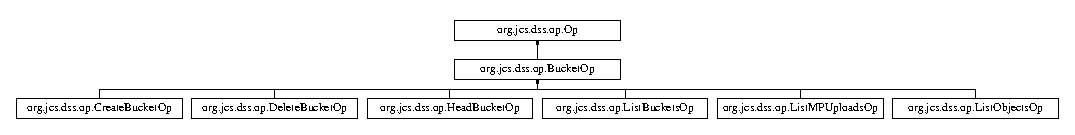
\includegraphics[height=1.372549cm]{classorg_1_1jcs_1_1dss_1_1op_1_1BucketOp}
\end{center}
\end{figure}
\subsection*{Public Member Functions}
\begin{DoxyCompactItemize}
\item 
\hyperlink{classorg_1_1jcs_1_1dss_1_1op_1_1BucketOp_ab023608e035a18fc468451ba2a65e049}{Bucket\+Op} (Dss\+Connection conn, String bucket\+Name)\hypertarget{classorg_1_1jcs_1_1dss_1_1op_1_1BucketOp_ab023608e035a18fc468451ba2a65e049}{}\label{classorg_1_1jcs_1_1dss_1_1op_1_1BucketOp_ab023608e035a18fc468451ba2a65e049}

\begin{DoxyCompactList}\small\item\em Constructors. \end{DoxyCompactList}\item 
Response \hyperlink{classorg_1_1jcs_1_1dss_1_1op_1_1BucketOp_a192b45bd81daa20a4e091f756d5df36c}{execute} ()  throws Exception 
\begin{DoxyCompactList}\small\item\em Executes the method requested by user. \end{DoxyCompactList}\item 
Object \hyperlink{classorg_1_1jcs_1_1dss_1_1op_1_1BucketOp_a0fd5f6a5286e3347f539a344480caadc}{process\+Result} (Object result)  throws I\+O\+Exception\hypertarget{classorg_1_1jcs_1_1dss_1_1op_1_1BucketOp_a0fd5f6a5286e3347f539a344480caadc}{}\label{classorg_1_1jcs_1_1dss_1_1op_1_1BucketOp_a0fd5f6a5286e3347f539a344480caadc}

\begin{DoxyCompactList}\small\item\em Processes the final result. \end{DoxyCompactList}\end{DoxyCompactItemize}
\subsection*{Additional Inherited Members}


\subsection{Detailed Description}
Head Class for all operations related to bucket. 

\subsection{Member Function Documentation}
\index{org\+::jcs\+::dss\+::op\+::\+Bucket\+Op@{org\+::jcs\+::dss\+::op\+::\+Bucket\+Op}!execute@{execute}}
\index{execute@{execute}!org\+::jcs\+::dss\+::op\+::\+Bucket\+Op@{org\+::jcs\+::dss\+::op\+::\+Bucket\+Op}}
\subsubsection[{\texorpdfstring{execute()}{execute()}}]{\setlength{\rightskip}{0pt plus 5cm}Response org.\+jcs.\+dss.\+op.\+Bucket\+Op.\+execute (
\begin{DoxyParamCaption}
{}
\end{DoxyParamCaption}
) throws Exception\hspace{0.3cm}{\ttfamily [inline]}}\hypertarget{classorg_1_1jcs_1_1dss_1_1op_1_1BucketOp_a192b45bd81daa20a4e091f756d5df36c}{}\label{classorg_1_1jcs_1_1dss_1_1op_1_1BucketOp_a192b45bd81daa20a4e091f756d5df36c}


Executes the method requested by user. 

\begin{DoxyReturn}{Returns}
Response \+: Gets response object returned from \hyperlink{classorg_1_1jcs_1_1dss_1_1op_1_1Op_a8502896422a70d8e8f712b57490b1a91}{make\+Request()} 
\end{DoxyReturn}

\begin{DoxyExceptions}{Exceptions}
{\em Exception} & \\
\hline
\end{DoxyExceptions}


The documentation for this class was generated from the following file\+:\begin{DoxyCompactItemize}
\item 
Bucket\+Op.\+java\end{DoxyCompactItemize}

\hypertarget{classorg_1_1jcs_1_1dss_1_1op_1_1CancelMPUploadOp}{}\section{org.\+jcs.\+dss.\+op.\+Cancel\+M\+P\+Upload\+Op Class Reference}
\label{classorg_1_1jcs_1_1dss_1_1op_1_1CancelMPUploadOp}\index{org.\+jcs.\+dss.\+op.\+Cancel\+M\+P\+Upload\+Op@{org.\+jcs.\+dss.\+op.\+Cancel\+M\+P\+Upload\+Op}}


Sets constructors like http\+Method, query\+String, etc to Cancel a multipart upload.  


Inheritance diagram for org.\+jcs.\+dss.\+op.\+Cancel\+M\+P\+Upload\+Op\+:\begin{figure}[H]
\begin{center}
\leavevmode
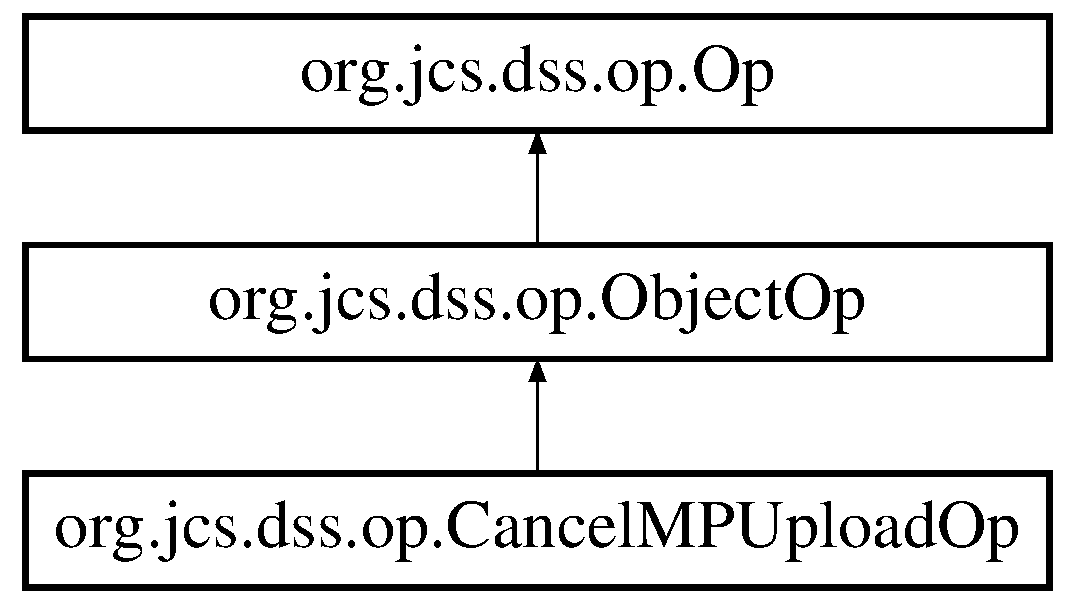
\includegraphics[height=3.000000cm]{classorg_1_1jcs_1_1dss_1_1op_1_1CancelMPUploadOp}
\end{center}
\end{figure}
\subsection*{Public Member Functions}
\begin{DoxyCompactItemize}
\item 
\hyperlink{classorg_1_1jcs_1_1dss_1_1op_1_1CancelMPUploadOp_acaad0e61e579534a67fc4bdd47291750}{Cancel\+M\+P\+Upload\+Op} (Dss\+Connection conn, String bucket\+Name, String object\+Name, String upload\+Id)\hypertarget{classorg_1_1jcs_1_1dss_1_1op_1_1CancelMPUploadOp_acaad0e61e579534a67fc4bdd47291750}{}\label{classorg_1_1jcs_1_1dss_1_1op_1_1CancelMPUploadOp_acaad0e61e579534a67fc4bdd47291750}

\begin{DoxyCompactList}\small\item\em Constructors. \end{DoxyCompactList}\end{DoxyCompactItemize}
\subsection*{Additional Inherited Members}


\subsection{Detailed Description}
Sets constructors like http\+Method, query\+String, etc to Cancel a multipart upload. 

The documentation for this class was generated from the following file\+:\begin{DoxyCompactItemize}
\item 
Cancel\+M\+P\+Upload\+Op.\+java\end{DoxyCompactItemize}

\hypertarget{classorg_1_1jcs_1_1dss_1_1op_1_1CompleteMPUploadOp}{}\section{org.\+jcs.\+dss.\+op.\+Complete\+M\+P\+Upload\+Op Class Reference}
\label{classorg_1_1jcs_1_1dss_1_1op_1_1CompleteMPUploadOp}\index{org.\+jcs.\+dss.\+op.\+Complete\+M\+P\+Upload\+Op@{org.\+jcs.\+dss.\+op.\+Complete\+M\+P\+Upload\+Op}}


Class to execute Complete multipart upload.  


Inheritance diagram for org.\+jcs.\+dss.\+op.\+Complete\+M\+P\+Upload\+Op\+:\begin{figure}[H]
\begin{center}
\leavevmode
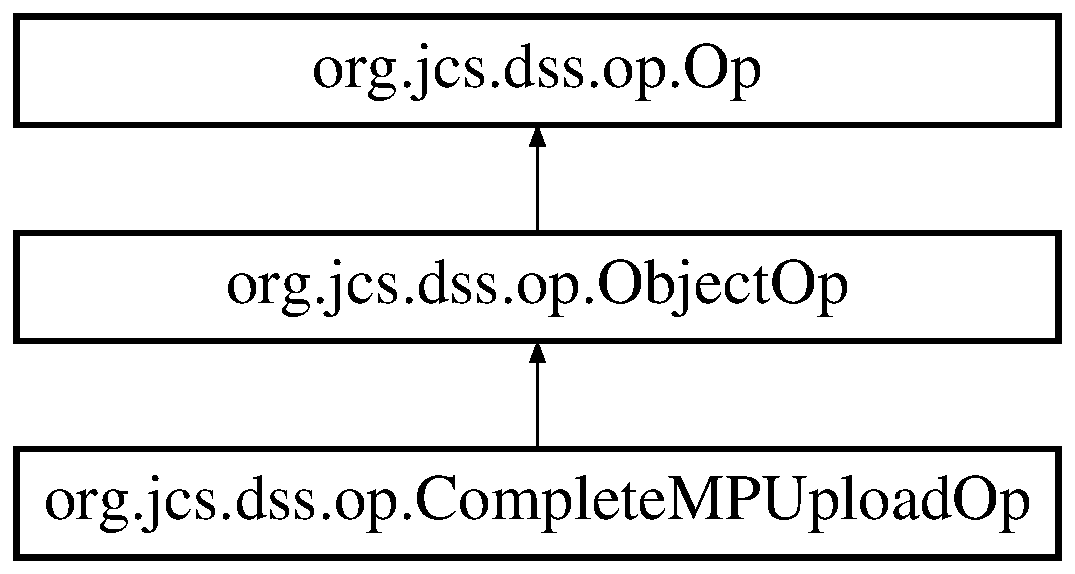
\includegraphics[height=3.000000cm]{classorg_1_1jcs_1_1dss_1_1op_1_1CompleteMPUploadOp}
\end{center}
\end{figure}
\subsection*{Public Member Functions}
\begin{DoxyCompactItemize}
\item 
\hyperlink{classorg_1_1jcs_1_1dss_1_1op_1_1CompleteMPUploadOp_a8736c298c1dca59b038fd44ef2eec39a}{Complete\+M\+P\+Upload\+Op} (Dss\+Connection conn, String bucket\+Name, String object\+Name, String upload\+Id, String multipart\+Upload)\hypertarget{classorg_1_1jcs_1_1dss_1_1op_1_1CompleteMPUploadOp_a8736c298c1dca59b038fd44ef2eec39a}{}\label{classorg_1_1jcs_1_1dss_1_1op_1_1CompleteMPUploadOp_a8736c298c1dca59b038fd44ef2eec39a}

\begin{DoxyCompactList}\small\item\em Constructors. \end{DoxyCompactList}\item 
Response \hyperlink{classorg_1_1jcs_1_1dss_1_1op_1_1CompleteMPUploadOp_a24540ef77bd0fb6424888b3a6ea2b223}{execute} ()  throws Exception 
\begin{DoxyCompactList}\small\item\em Executes the method requested by user. \end{DoxyCompactList}\item 
Response \hyperlink{classorg_1_1jcs_1_1dss_1_1op_1_1CompleteMPUploadOp_adefa48266f195cbd6baf6d6dd6d093f3}{make\+Request} ()  throws Exception 
\begin{DoxyCompactList}\small\item\em This method first gets signature, sets http\+Headers and then gets Response object. \end{DoxyCompactList}\item 
Object \hyperlink{classorg_1_1jcs_1_1dss_1_1op_1_1CompleteMPUploadOp_a9a5e5ba31cea414e044dce4ba51b3b64}{process\+Result} (Object resp)  throws I\+O\+Exception
\begin{DoxyCompactList}\small\item\em This method extracts information such as key, E\+Tag etc from Input\+Stream got from Server. \end{DoxyCompactList}\end{DoxyCompactItemize}
\subsection*{Additional Inherited Members}


\subsection{Detailed Description}
Class to execute Complete multipart upload. 

\subsection{Member Function Documentation}
\index{org\+::jcs\+::dss\+::op\+::\+Complete\+M\+P\+Upload\+Op@{org\+::jcs\+::dss\+::op\+::\+Complete\+M\+P\+Upload\+Op}!execute@{execute}}
\index{execute@{execute}!org\+::jcs\+::dss\+::op\+::\+Complete\+M\+P\+Upload\+Op@{org\+::jcs\+::dss\+::op\+::\+Complete\+M\+P\+Upload\+Op}}
\subsubsection[{\texorpdfstring{execute()}{execute()}}]{\setlength{\rightskip}{0pt plus 5cm}Response org.\+jcs.\+dss.\+op.\+Complete\+M\+P\+Upload\+Op.\+execute (
\begin{DoxyParamCaption}
{}
\end{DoxyParamCaption}
) throws Exception\hspace{0.3cm}{\ttfamily [inline]}}\hypertarget{classorg_1_1jcs_1_1dss_1_1op_1_1CompleteMPUploadOp_a24540ef77bd0fb6424888b3a6ea2b223}{}\label{classorg_1_1jcs_1_1dss_1_1op_1_1CompleteMPUploadOp_a24540ef77bd0fb6424888b3a6ea2b223}


Executes the method requested by user. 

\begin{DoxyReturn}{Returns}
Response \+: Gets response object returned from \hyperlink{classorg_1_1jcs_1_1dss_1_1op_1_1CompleteMPUploadOp_adefa48266f195cbd6baf6d6dd6d093f3}{make\+Request()} 
\end{DoxyReturn}

\begin{DoxyExceptions}{Exceptions}
{\em Exception} & \\
\hline
\end{DoxyExceptions}
\index{org\+::jcs\+::dss\+::op\+::\+Complete\+M\+P\+Upload\+Op@{org\+::jcs\+::dss\+::op\+::\+Complete\+M\+P\+Upload\+Op}!make\+Request@{make\+Request}}
\index{make\+Request@{make\+Request}!org\+::jcs\+::dss\+::op\+::\+Complete\+M\+P\+Upload\+Op@{org\+::jcs\+::dss\+::op\+::\+Complete\+M\+P\+Upload\+Op}}
\subsubsection[{\texorpdfstring{make\+Request()}{makeRequest()}}]{\setlength{\rightskip}{0pt plus 5cm}Response org.\+jcs.\+dss.\+op.\+Complete\+M\+P\+Upload\+Op.\+make\+Request (
\begin{DoxyParamCaption}
{}
\end{DoxyParamCaption}
) throws Exception\hspace{0.3cm}{\ttfamily [inline]}}\hypertarget{classorg_1_1jcs_1_1dss_1_1op_1_1CompleteMPUploadOp_adefa48266f195cbd6baf6d6dd6d093f3}{}\label{classorg_1_1jcs_1_1dss_1_1op_1_1CompleteMPUploadOp_adefa48266f195cbd6baf6d6dd6d093f3}


This method first gets signature, sets http\+Headers and then gets Response object. 

\begin{DoxyReturn}{Returns}
Response \+: response object by calling put method under request class 
\end{DoxyReturn}
Creating object of Dss\+Auth to get signature \index{org\+::jcs\+::dss\+::op\+::\+Complete\+M\+P\+Upload\+Op@{org\+::jcs\+::dss\+::op\+::\+Complete\+M\+P\+Upload\+Op}!process\+Result@{process\+Result}}
\index{process\+Result@{process\+Result}!org\+::jcs\+::dss\+::op\+::\+Complete\+M\+P\+Upload\+Op@{org\+::jcs\+::dss\+::op\+::\+Complete\+M\+P\+Upload\+Op}}
\subsubsection[{\texorpdfstring{process\+Result(\+Object resp)}{processResult(Object resp)}}]{\setlength{\rightskip}{0pt plus 5cm}Object org.\+jcs.\+dss.\+op.\+Complete\+M\+P\+Upload\+Op.\+process\+Result (
\begin{DoxyParamCaption}
\item[{Object}]{resp}
\end{DoxyParamCaption}
) throws I\+O\+Exception\hspace{0.3cm}{\ttfamily [inline]}}\hypertarget{classorg_1_1jcs_1_1dss_1_1op_1_1CompleteMPUploadOp_a9a5e5ba31cea414e044dce4ba51b3b64}{}\label{classorg_1_1jcs_1_1dss_1_1op_1_1CompleteMPUploadOp_a9a5e5ba31cea414e044dce4ba51b3b64}


This method extracts information such as key, E\+Tag etc from Input\+Stream got from Server. 


\begin{DoxyParams}{Parameters}
{\em Response} & \+: Response message got from Request.\+put() \\
\hline
\end{DoxyParams}
\begin{DoxyReturn}{Returns}
Complete\+Multipart\+Upload\+Result \+: A class that contains all the information about a successful uploaded object 
\end{DoxyReturn}

\begin{DoxyExceptions}{Exceptions}
{\em I\+O\+Exception} & \\
\hline
\end{DoxyExceptions}


The documentation for this class was generated from the following file\+:\begin{DoxyCompactItemize}
\item 
Complete\+M\+P\+Upload\+Op.\+java\end{DoxyCompactItemize}

\hypertarget{classorg_1_1jcs_1_1dss_1_1op_1_1CopyObjectOp}{}\section{org.\+jcs.\+dss.\+op.\+Copy\+Object\+Op Class Reference}
\label{classorg_1_1jcs_1_1dss_1_1op_1_1CopyObjectOp}\index{org.\+jcs.\+dss.\+op.\+Copy\+Object\+Op@{org.\+jcs.\+dss.\+op.\+Copy\+Object\+Op}}


Class to execute method for copying Object from one bucket to another.  


Inheritance diagram for org.\+jcs.\+dss.\+op.\+Copy\+Object\+Op\+:\begin{figure}[H]
\begin{center}
\leavevmode
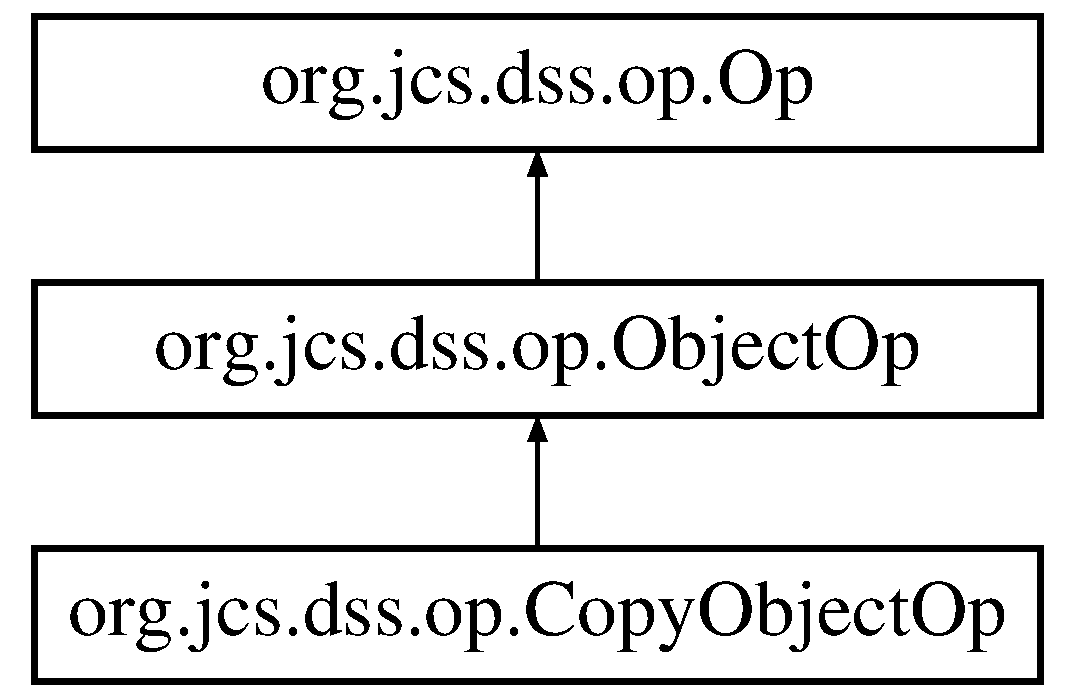
\includegraphics[height=3.000000cm]{classorg_1_1jcs_1_1dss_1_1op_1_1CopyObjectOp}
\end{center}
\end{figure}
\subsection*{Public Member Functions}
\begin{DoxyCompactItemize}
\item 
\hyperlink{classorg_1_1jcs_1_1dss_1_1op_1_1CopyObjectOp_a1c6f7605c588295606ee7b073571f688}{Copy\+Object\+Op} (Dss\+Connection conn, String bucket\+Name, String object\+Name, String Jcs\+Copy\+Path)\hypertarget{classorg_1_1jcs_1_1dss_1_1op_1_1CopyObjectOp_a1c6f7605c588295606ee7b073571f688}{}\label{classorg_1_1jcs_1_1dss_1_1op_1_1CopyObjectOp_a1c6f7605c588295606ee7b073571f688}

\begin{DoxyCompactList}\small\item\em Constructors. \end{DoxyCompactList}\item 
Response \hyperlink{classorg_1_1jcs_1_1dss_1_1op_1_1CopyObjectOp_a025ad8a7df5e040398bba72d1ee50438}{execute} ()  throws Exception 
\begin{DoxyCompactList}\small\item\em Executes the method requested by user. \end{DoxyCompactList}\item 
Response \hyperlink{classorg_1_1jcs_1_1dss_1_1op_1_1CopyObjectOp_ad9ac1d7eaf2ab0be9893b273e955b8e4}{put\+Headers} ()  throws Exception 
\begin{DoxyCompactList}\small\item\em This method assign additional headers which are not present in Op.\+make\+Requests() \end{DoxyCompactList}\item 
Object \hyperlink{classorg_1_1jcs_1_1dss_1_1op_1_1CopyObjectOp_adceba3616fa9df2c95f22c8979295b78}{process\+Result} (Object resp)  throws I\+O\+Exception
\begin{DoxyCompactList}\small\item\em This method extracts information about newly copied object such as Last\+Modified and E\+Tag from Input\+Stream got from Server. \end{DoxyCompactList}\end{DoxyCompactItemize}
\subsection*{Additional Inherited Members}


\subsection{Detailed Description}
Class to execute method for copying Object from one bucket to another. 

\subsection{Member Function Documentation}
\index{org\+::jcs\+::dss\+::op\+::\+Copy\+Object\+Op@{org\+::jcs\+::dss\+::op\+::\+Copy\+Object\+Op}!execute@{execute}}
\index{execute@{execute}!org\+::jcs\+::dss\+::op\+::\+Copy\+Object\+Op@{org\+::jcs\+::dss\+::op\+::\+Copy\+Object\+Op}}
\subsubsection[{\texorpdfstring{execute()}{execute()}}]{\setlength{\rightskip}{0pt plus 5cm}Response org.\+jcs.\+dss.\+op.\+Copy\+Object\+Op.\+execute (
\begin{DoxyParamCaption}
{}
\end{DoxyParamCaption}
) throws Exception\hspace{0.3cm}{\ttfamily [inline]}}\hypertarget{classorg_1_1jcs_1_1dss_1_1op_1_1CopyObjectOp_a025ad8a7df5e040398bba72d1ee50438}{}\label{classorg_1_1jcs_1_1dss_1_1op_1_1CopyObjectOp_a025ad8a7df5e040398bba72d1ee50438}


Executes the method requested by user. 

\begin{DoxyReturn}{Returns}
Response \+: Gets response object returned from \hyperlink{classorg_1_1jcs_1_1dss_1_1op_1_1CopyObjectOp_ad9ac1d7eaf2ab0be9893b273e955b8e4}{put\+Headers()} 
\end{DoxyReturn}

\begin{DoxyExceptions}{Exceptions}
{\em Exception} & \\
\hline
\end{DoxyExceptions}
\index{org\+::jcs\+::dss\+::op\+::\+Copy\+Object\+Op@{org\+::jcs\+::dss\+::op\+::\+Copy\+Object\+Op}!process\+Result@{process\+Result}}
\index{process\+Result@{process\+Result}!org\+::jcs\+::dss\+::op\+::\+Copy\+Object\+Op@{org\+::jcs\+::dss\+::op\+::\+Copy\+Object\+Op}}
\subsubsection[{\texorpdfstring{process\+Result(\+Object resp)}{processResult(Object resp)}}]{\setlength{\rightskip}{0pt plus 5cm}Object org.\+jcs.\+dss.\+op.\+Copy\+Object\+Op.\+process\+Result (
\begin{DoxyParamCaption}
\item[{Object}]{resp}
\end{DoxyParamCaption}
) throws I\+O\+Exception\hspace{0.3cm}{\ttfamily [inline]}}\hypertarget{classorg_1_1jcs_1_1dss_1_1op_1_1CopyObjectOp_adceba3616fa9df2c95f22c8979295b78}{}\label{classorg_1_1jcs_1_1dss_1_1op_1_1CopyObjectOp_adceba3616fa9df2c95f22c8979295b78}


This method extracts information about newly copied object such as Last\+Modified and E\+Tag from Input\+Stream got from Server. 


\begin{DoxyParams}{Parameters}
{\em Response} & \+: Response message got from Request.\+put() \\
\hline
\end{DoxyParams}
\begin{DoxyReturn}{Returns}
Copy\+Object\+Result \+: A class that contains information about a newly copied object 
\end{DoxyReturn}

\begin{DoxyExceptions}{Exceptions}
{\em I\+O\+Exception} & \\
\hline
\end{DoxyExceptions}
\index{org\+::jcs\+::dss\+::op\+::\+Copy\+Object\+Op@{org\+::jcs\+::dss\+::op\+::\+Copy\+Object\+Op}!put\+Headers@{put\+Headers}}
\index{put\+Headers@{put\+Headers}!org\+::jcs\+::dss\+::op\+::\+Copy\+Object\+Op@{org\+::jcs\+::dss\+::op\+::\+Copy\+Object\+Op}}
\subsubsection[{\texorpdfstring{put\+Headers()}{putHeaders()}}]{\setlength{\rightskip}{0pt plus 5cm}Response org.\+jcs.\+dss.\+op.\+Copy\+Object\+Op.\+put\+Headers (
\begin{DoxyParamCaption}
{}
\end{DoxyParamCaption}
) throws Exception\hspace{0.3cm}{\ttfamily [inline]}}\hypertarget{classorg_1_1jcs_1_1dss_1_1op_1_1CopyObjectOp_ad9ac1d7eaf2ab0be9893b273e955b8e4}{}\label{classorg_1_1jcs_1_1dss_1_1op_1_1CopyObjectOp_ad9ac1d7eaf2ab0be9893b273e955b8e4}


This method assign additional headers which are not present in Op.\+make\+Requests() 

\begin{DoxyReturn}{Returns}
Response \+: Gets response object returned from \hyperlink{classorg_1_1jcs_1_1dss_1_1op_1_1Op_a8502896422a70d8e8f712b57490b1a91}{make\+Request()} 
\end{DoxyReturn}

\begin{DoxyExceptions}{Exceptions}
{\em Exception} & \\
\hline
\end{DoxyExceptions}


The documentation for this class was generated from the following file\+:\begin{DoxyCompactItemize}
\item 
Copy\+Object\+Op.\+java\end{DoxyCompactItemize}

\hypertarget{classorg_1_1jcs_1_1dss_1_1op_1_1CreateBucketOp}{}\section{org.\+jcs.\+dss.\+op.\+Create\+Bucket\+Op Class Reference}
\label{classorg_1_1jcs_1_1dss_1_1op_1_1CreateBucketOp}\index{org.\+jcs.\+dss.\+op.\+Create\+Bucket\+Op@{org.\+jcs.\+dss.\+op.\+Create\+Bucket\+Op}}


Class to create a new bucket.  


Inheritance diagram for org.\+jcs.\+dss.\+op.\+Create\+Bucket\+Op\+:\begin{figure}[H]
\begin{center}
\leavevmode
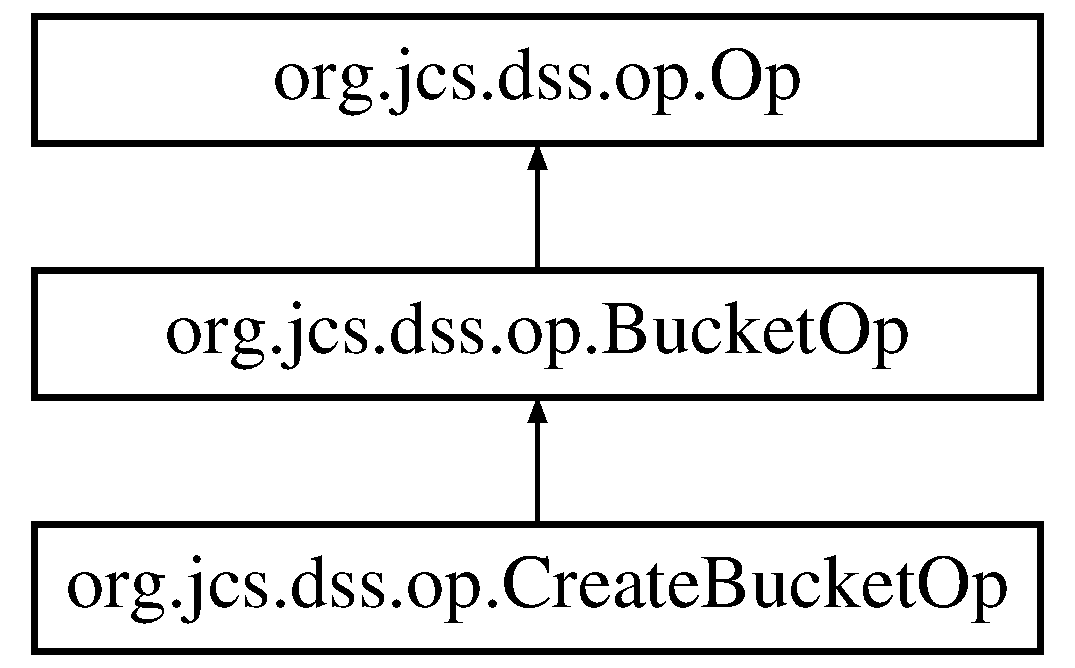
\includegraphics[height=3.000000cm]{classorg_1_1jcs_1_1dss_1_1op_1_1CreateBucketOp}
\end{center}
\end{figure}
\subsection*{Public Member Functions}
\begin{DoxyCompactItemize}
\item 
\hyperlink{classorg_1_1jcs_1_1dss_1_1op_1_1CreateBucketOp_a723a84d7217ac9cb9df50fff6a84c371}{Create\+Bucket\+Op} (Dss\+Connection conn, String bucket\+Name)\hypertarget{classorg_1_1jcs_1_1dss_1_1op_1_1CreateBucketOp_a723a84d7217ac9cb9df50fff6a84c371}{}\label{classorg_1_1jcs_1_1dss_1_1op_1_1CreateBucketOp_a723a84d7217ac9cb9df50fff6a84c371}

\begin{DoxyCompactList}\small\item\em Constructors. \end{DoxyCompactList}\item 
Object \hyperlink{classorg_1_1jcs_1_1dss_1_1op_1_1CreateBucketOp_ad9317afb5adad4749a2e2060c768ddb3}{process\+Result} (Object bucket\+Name)
\begin{DoxyCompactList}\small\item\em Class to put creation date and return the bucket object. \end{DoxyCompactList}\end{DoxyCompactItemize}
\subsection*{Additional Inherited Members}


\subsection{Detailed Description}
Class to create a new bucket. 

\subsection{Member Function Documentation}
\index{org\+::jcs\+::dss\+::op\+::\+Create\+Bucket\+Op@{org\+::jcs\+::dss\+::op\+::\+Create\+Bucket\+Op}!process\+Result@{process\+Result}}
\index{process\+Result@{process\+Result}!org\+::jcs\+::dss\+::op\+::\+Create\+Bucket\+Op@{org\+::jcs\+::dss\+::op\+::\+Create\+Bucket\+Op}}
\subsubsection[{\texorpdfstring{process\+Result(\+Object bucket\+Name)}{processResult(Object bucketName)}}]{\setlength{\rightskip}{0pt plus 5cm}Object org.\+jcs.\+dss.\+op.\+Create\+Bucket\+Op.\+process\+Result (
\begin{DoxyParamCaption}
\item[{Object}]{bucket\+Name}
\end{DoxyParamCaption}
)\hspace{0.3cm}{\ttfamily [inline]}}\hypertarget{classorg_1_1jcs_1_1dss_1_1op_1_1CreateBucketOp_ad9317afb5adad4749a2e2060c768ddb3}{}\label{classorg_1_1jcs_1_1dss_1_1op_1_1CreateBucketOp_ad9317afb5adad4749a2e2060c768ddb3}


Class to put creation date and return the bucket object. 


\begin{DoxyParams}{Parameters}
{\em Bucket\+Name} & \+: Name of new bucket entered by user \\
\hline
\end{DoxyParams}
\begin{DoxyReturn}{Returns}
Bucket \+: An Object of bucket class having details of bucket name and creation date 
\end{DoxyReturn}


The documentation for this class was generated from the following file\+:\begin{DoxyCompactItemize}
\item 
Create\+Bucket\+Op.\+java\end{DoxyCompactItemize}

\hypertarget{classorg_1_1jcs_1_1dss_1_1op_1_1DeleteBucketOp}{}\section{org.\+jcs.\+dss.\+op.\+Delete\+Bucket\+Op Class Reference}
\label{classorg_1_1jcs_1_1dss_1_1op_1_1DeleteBucketOp}\index{org.\+jcs.\+dss.\+op.\+Delete\+Bucket\+Op@{org.\+jcs.\+dss.\+op.\+Delete\+Bucket\+Op}}


Class to Delete an existing bucket.  


Inheritance diagram for org.\+jcs.\+dss.\+op.\+Delete\+Bucket\+Op\+:\begin{figure}[H]
\begin{center}
\leavevmode
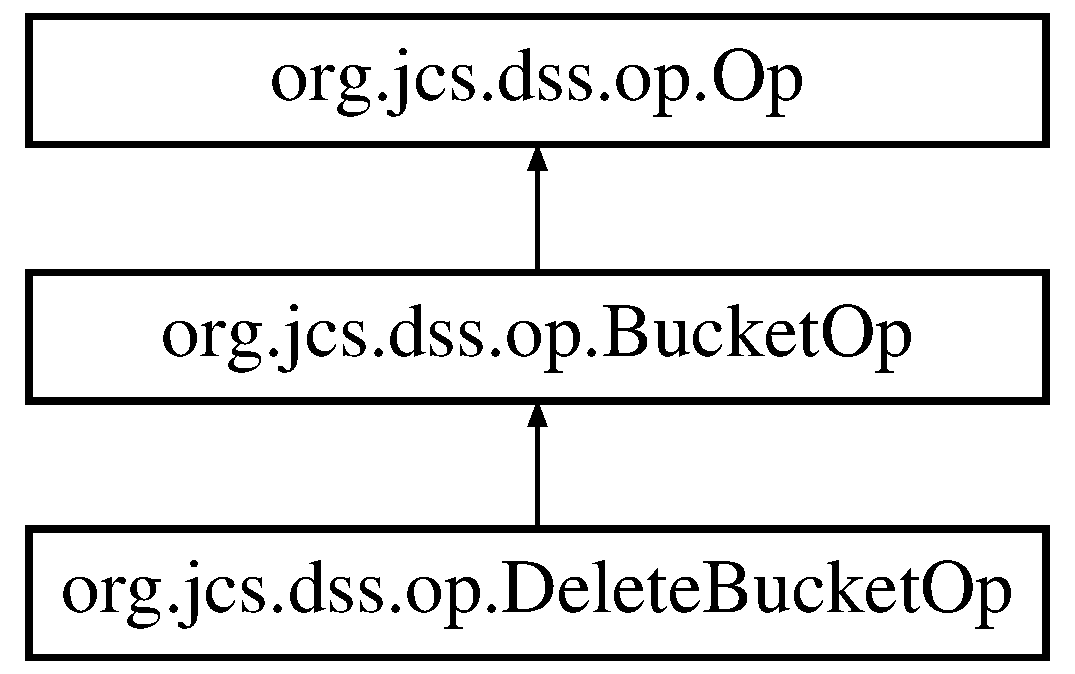
\includegraphics[height=3.000000cm]{classorg_1_1jcs_1_1dss_1_1op_1_1DeleteBucketOp}
\end{center}
\end{figure}
\subsection*{Public Member Functions}
\begin{DoxyCompactItemize}
\item 
\hyperlink{classorg_1_1jcs_1_1dss_1_1op_1_1DeleteBucketOp_a9e2669a82a1d8598968bedfc1e8e79f0}{Delete\+Bucket\+Op} (Dss\+Connection conn, String bucket\+Name)\hypertarget{classorg_1_1jcs_1_1dss_1_1op_1_1DeleteBucketOp_a9e2669a82a1d8598968bedfc1e8e79f0}{}\label{classorg_1_1jcs_1_1dss_1_1op_1_1DeleteBucketOp_a9e2669a82a1d8598968bedfc1e8e79f0}

\begin{DoxyCompactList}\small\item\em Constructors. \end{DoxyCompactList}\end{DoxyCompactItemize}
\subsection*{Additional Inherited Members}


\subsection{Detailed Description}
Class to Delete an existing bucket. 

The documentation for this class was generated from the following file\+:\begin{DoxyCompactItemize}
\item 
Delete\+Bucket\+Op.\+java\end{DoxyCompactItemize}

\hypertarget{classorg_1_1jcs_1_1dss_1_1op_1_1DeleteObjectOp}{}\section{org.\+jcs.\+dss.\+op.\+Delete\+Object\+Op Class Reference}
\label{classorg_1_1jcs_1_1dss_1_1op_1_1DeleteObjectOp}\index{org.\+jcs.\+dss.\+op.\+Delete\+Object\+Op@{org.\+jcs.\+dss.\+op.\+Delete\+Object\+Op}}


Class to Delete an existing key inside the requested bucket.  


Inheritance diagram for org.\+jcs.\+dss.\+op.\+Delete\+Object\+Op\+:\begin{figure}[H]
\begin{center}
\leavevmode
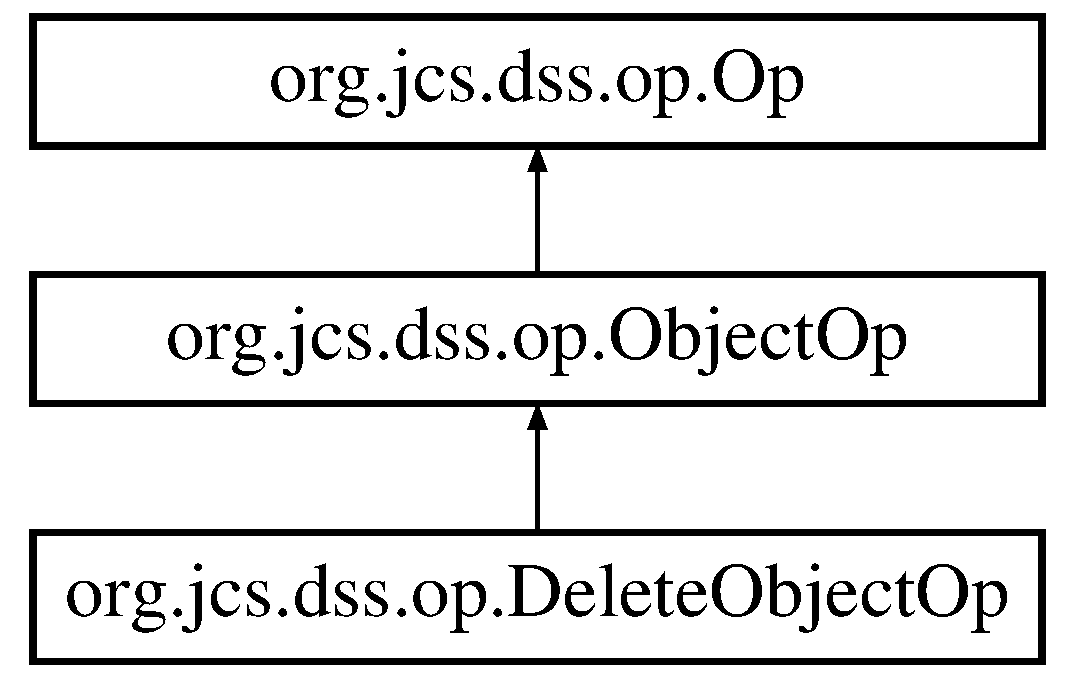
\includegraphics[height=3.000000cm]{classorg_1_1jcs_1_1dss_1_1op_1_1DeleteObjectOp}
\end{center}
\end{figure}
\subsection*{Public Member Functions}
\begin{DoxyCompactItemize}
\item 
\hyperlink{classorg_1_1jcs_1_1dss_1_1op_1_1DeleteObjectOp_a4971df5680e8bcd19bb577227c1bf37a}{Delete\+Object\+Op} (Dss\+Connection conn, String bucket\+Name, String object\+Name)\hypertarget{classorg_1_1jcs_1_1dss_1_1op_1_1DeleteObjectOp_a4971df5680e8bcd19bb577227c1bf37a}{}\label{classorg_1_1jcs_1_1dss_1_1op_1_1DeleteObjectOp_a4971df5680e8bcd19bb577227c1bf37a}

\begin{DoxyCompactList}\small\item\em Constructors. \end{DoxyCompactList}\end{DoxyCompactItemize}
\subsection*{Additional Inherited Members}


\subsection{Detailed Description}
Class to Delete an existing key inside the requested bucket. 

The documentation for this class was generated from the following file\+:\begin{DoxyCompactItemize}
\item 
Delete\+Object\+Op.\+java\end{DoxyCompactItemize}

\hypertarget{classorg_1_1jcs_1_1dss_1_1op_1_1GetObjectDetailOp}{}\section{org.\+jcs.\+dss.\+op.\+Get\+Object\+Detail\+Op Class Reference}
\label{classorg_1_1jcs_1_1dss_1_1op_1_1GetObjectDetailOp}\index{org.\+jcs.\+dss.\+op.\+Get\+Object\+Detail\+Op@{org.\+jcs.\+dss.\+op.\+Get\+Object\+Detail\+Op}}


Class to get details regarding E\+Tag, content Length etc of the requested object.  


Inheritance diagram for org.\+jcs.\+dss.\+op.\+Get\+Object\+Detail\+Op\+:\begin{figure}[H]
\begin{center}
\leavevmode
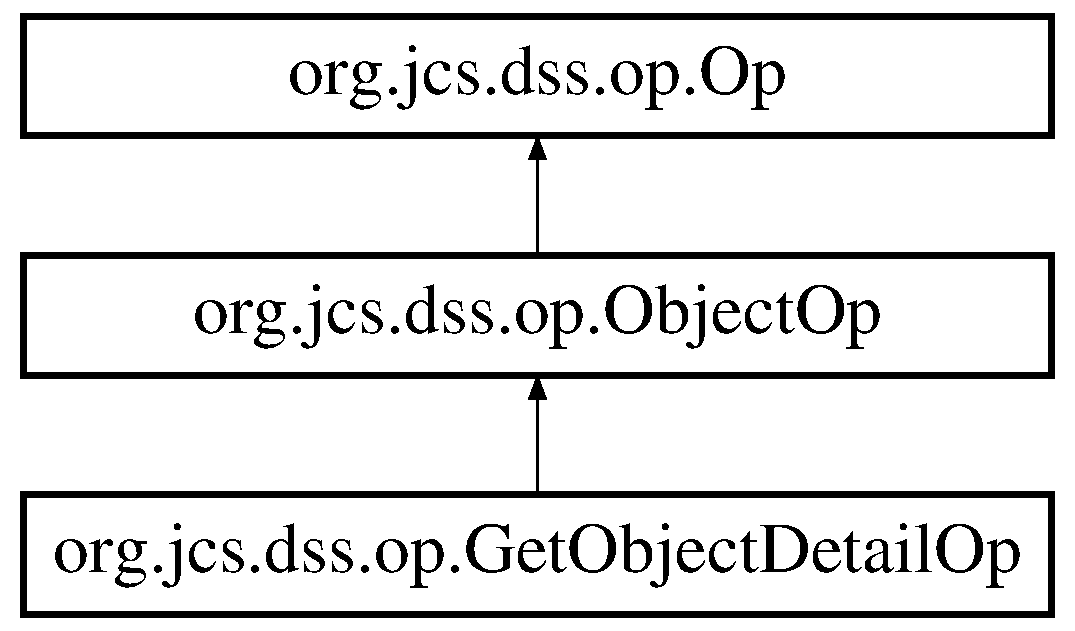
\includegraphics[height=3.000000cm]{classorg_1_1jcs_1_1dss_1_1op_1_1GetObjectDetailOp}
\end{center}
\end{figure}
\subsection*{Public Member Functions}
\begin{DoxyCompactItemize}
\item 
\hyperlink{classorg_1_1jcs_1_1dss_1_1op_1_1GetObjectDetailOp_a282d865ccd75dddc2b956059a6171a75}{Get\+Object\+Detail\+Op} (Dss\+Connection conn, String bucket\+Name, String object\+Name)\hypertarget{classorg_1_1jcs_1_1dss_1_1op_1_1GetObjectDetailOp_a282d865ccd75dddc2b956059a6171a75}{}\label{classorg_1_1jcs_1_1dss_1_1op_1_1GetObjectDetailOp_a282d865ccd75dddc2b956059a6171a75}

\begin{DoxyCompactList}\small\item\em Constructors. \end{DoxyCompactList}\item 
Object \hyperlink{classorg_1_1jcs_1_1dss_1_1op_1_1GetObjectDetailOp_a5498a9b8d534ffc0a74e2ecad3833fdd}{process\+Result} (Object resp)
\begin{DoxyCompactList}\small\item\em This method extracts information from headers got from server. \end{DoxyCompactList}\end{DoxyCompactItemize}
\subsection*{Additional Inherited Members}


\subsection{Detailed Description}
Class to get details regarding E\+Tag, content Length etc of the requested object. 

\subsection{Member Function Documentation}
\index{org\+::jcs\+::dss\+::op\+::\+Get\+Object\+Detail\+Op@{org\+::jcs\+::dss\+::op\+::\+Get\+Object\+Detail\+Op}!process\+Result@{process\+Result}}
\index{process\+Result@{process\+Result}!org\+::jcs\+::dss\+::op\+::\+Get\+Object\+Detail\+Op@{org\+::jcs\+::dss\+::op\+::\+Get\+Object\+Detail\+Op}}
\subsubsection[{\texorpdfstring{process\+Result(\+Object resp)}{processResult(Object resp)}}]{\setlength{\rightskip}{0pt plus 5cm}Object org.\+jcs.\+dss.\+op.\+Get\+Object\+Detail\+Op.\+process\+Result (
\begin{DoxyParamCaption}
\item[{Object}]{resp}
\end{DoxyParamCaption}
)\hspace{0.3cm}{\ttfamily [inline]}}\hypertarget{classorg_1_1jcs_1_1dss_1_1op_1_1GetObjectDetailOp_a5498a9b8d534ffc0a74e2ecad3833fdd}{}\label{classorg_1_1jcs_1_1dss_1_1op_1_1GetObjectDetailOp_a5498a9b8d534ffc0a74e2ecad3833fdd}


This method extracts information from headers got from server. 


\begin{DoxyParams}{Parameters}
{\em Response} & \+: Response message got from Request.\+request() \\
\hline
\end{DoxyParams}
\begin{DoxyReturn}{Returns}
Objectdata \+: Object of a class containing information about requested key 
\end{DoxyReturn}


The documentation for this class was generated from the following file\+:\begin{DoxyCompactItemize}
\item 
Get\+Object\+Detail\+Op.\+java\end{DoxyCompactItemize}

\hypertarget{classorg_1_1jcs_1_1dss_1_1op_1_1GetObjectOp}{}\section{org.\+jcs.\+dss.\+op.\+Get\+Object\+Op Class Reference}
\label{classorg_1_1jcs_1_1dss_1_1op_1_1GetObjectOp}\index{org.\+jcs.\+dss.\+op.\+Get\+Object\+Op@{org.\+jcs.\+dss.\+op.\+Get\+Object\+Op}}


Class to download object file from request key to desired path.  


Inheritance diagram for org.\+jcs.\+dss.\+op.\+Get\+Object\+Op\+:\begin{figure}[H]
\begin{center}
\leavevmode
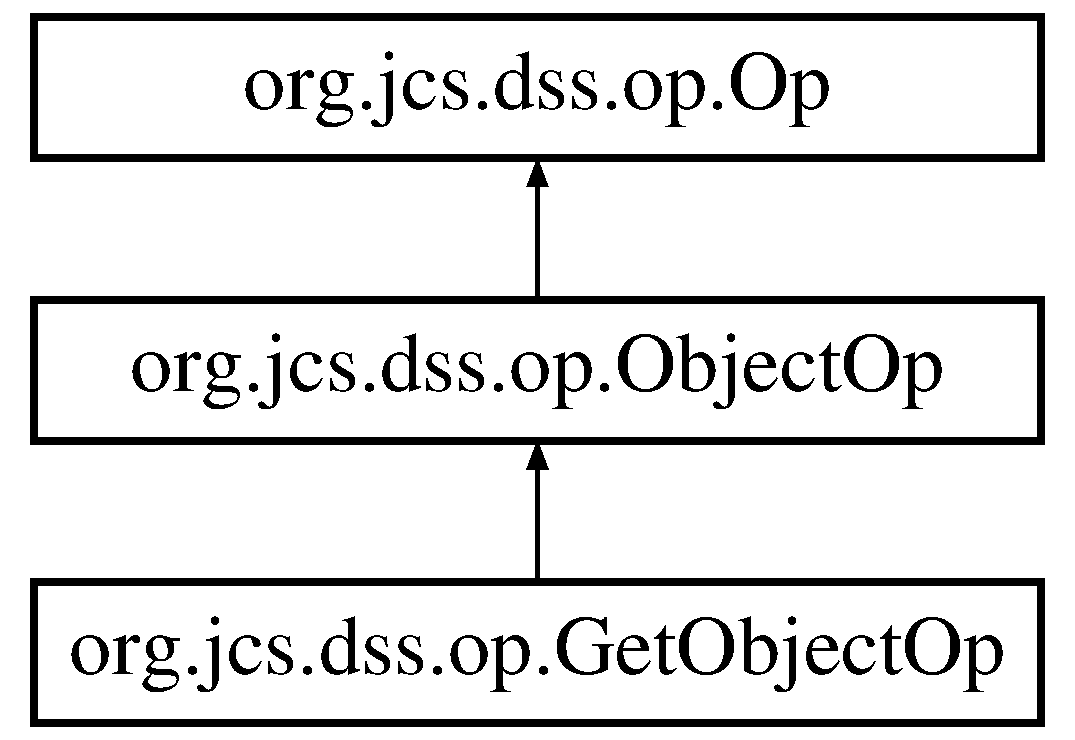
\includegraphics[height=3.000000cm]{classorg_1_1jcs_1_1dss_1_1op_1_1GetObjectOp}
\end{center}
\end{figure}
\subsection*{Public Member Functions}
\begin{DoxyCompactItemize}
\item 
\hyperlink{classorg_1_1jcs_1_1dss_1_1op_1_1GetObjectOp_a3c6cbde6de75cd9b9c30fd3bdffdbbf5}{Get\+Object\+Op} (Dss\+Connection conn, String bucket\+Name, String object\+Name, String filepath)\hypertarget{classorg_1_1jcs_1_1dss_1_1op_1_1GetObjectOp_a3c6cbde6de75cd9b9c30fd3bdffdbbf5}{}\label{classorg_1_1jcs_1_1dss_1_1op_1_1GetObjectOp_a3c6cbde6de75cd9b9c30fd3bdffdbbf5}

\begin{DoxyCompactList}\small\item\em Constructors. \end{DoxyCompactList}\item 
Response \hyperlink{classorg_1_1jcs_1_1dss_1_1op_1_1GetObjectOp_a4fa98961dbe836640650a0eeaf1ae330}{execute} ()  throws Exception 
\begin{DoxyCompactList}\small\item\em Executes the method requested by user. \end{DoxyCompactList}\item 
Response \hyperlink{classorg_1_1jcs_1_1dss_1_1op_1_1GetObjectOp_a9323461b3d235ccdd505b09c97e6b796}{make\+Request} ()  throws Exception 
\begin{DoxyCompactList}\small\item\em This method first gets signature, sets http\+Headers and then gets Response object. \end{DoxyCompactList}\item 
Object \hyperlink{classorg_1_1jcs_1_1dss_1_1op_1_1GetObjectOp_a041a512683b6e12e3da821e680f5b805}{process\+Result} (Object resp)  throws I\+O\+Exception
\begin{DoxyCompactList}\small\item\em Process final step to download file to desired path. \end{DoxyCompactList}\end{DoxyCompactItemize}
\subsection*{Additional Inherited Members}


\subsection{Detailed Description}
Class to download object file from request key to desired path. 

\subsection{Member Function Documentation}
\index{org\+::jcs\+::dss\+::op\+::\+Get\+Object\+Op@{org\+::jcs\+::dss\+::op\+::\+Get\+Object\+Op}!execute@{execute}}
\index{execute@{execute}!org\+::jcs\+::dss\+::op\+::\+Get\+Object\+Op@{org\+::jcs\+::dss\+::op\+::\+Get\+Object\+Op}}
\subsubsection[{\texorpdfstring{execute()}{execute()}}]{\setlength{\rightskip}{0pt plus 5cm}Response org.\+jcs.\+dss.\+op.\+Get\+Object\+Op.\+execute (
\begin{DoxyParamCaption}
{}
\end{DoxyParamCaption}
) throws Exception\hspace{0.3cm}{\ttfamily [inline]}}\hypertarget{classorg_1_1jcs_1_1dss_1_1op_1_1GetObjectOp_a4fa98961dbe836640650a0eeaf1ae330}{}\label{classorg_1_1jcs_1_1dss_1_1op_1_1GetObjectOp_a4fa98961dbe836640650a0eeaf1ae330}


Executes the method requested by user. 

\begin{DoxyReturn}{Returns}
Response \+: Gets response object returned from \hyperlink{classorg_1_1jcs_1_1dss_1_1op_1_1GetObjectOp_a9323461b3d235ccdd505b09c97e6b796}{make\+Request()} 
\end{DoxyReturn}

\begin{DoxyExceptions}{Exceptions}
{\em Exception} & \\
\hline
\end{DoxyExceptions}
\index{org\+::jcs\+::dss\+::op\+::\+Get\+Object\+Op@{org\+::jcs\+::dss\+::op\+::\+Get\+Object\+Op}!make\+Request@{make\+Request}}
\index{make\+Request@{make\+Request}!org\+::jcs\+::dss\+::op\+::\+Get\+Object\+Op@{org\+::jcs\+::dss\+::op\+::\+Get\+Object\+Op}}
\subsubsection[{\texorpdfstring{make\+Request()}{makeRequest()}}]{\setlength{\rightskip}{0pt plus 5cm}Response org.\+jcs.\+dss.\+op.\+Get\+Object\+Op.\+make\+Request (
\begin{DoxyParamCaption}
{}
\end{DoxyParamCaption}
) throws Exception\hspace{0.3cm}{\ttfamily [inline]}}\hypertarget{classorg_1_1jcs_1_1dss_1_1op_1_1GetObjectOp_a9323461b3d235ccdd505b09c97e6b796}{}\label{classorg_1_1jcs_1_1dss_1_1op_1_1GetObjectOp_a9323461b3d235ccdd505b09c97e6b796}


This method first gets signature, sets http\+Headers and then gets Response object. 

\begin{DoxyReturn}{Returns}
Response \+: response object by calling request method under Request class 
\end{DoxyReturn}

\begin{DoxyExceptions}{Exceptions}
{\em Exception} & \\
\hline
\end{DoxyExceptions}
Creating object of Dss\+Auth to get signature \index{org\+::jcs\+::dss\+::op\+::\+Get\+Object\+Op@{org\+::jcs\+::dss\+::op\+::\+Get\+Object\+Op}!process\+Result@{process\+Result}}
\index{process\+Result@{process\+Result}!org\+::jcs\+::dss\+::op\+::\+Get\+Object\+Op@{org\+::jcs\+::dss\+::op\+::\+Get\+Object\+Op}}
\subsubsection[{\texorpdfstring{process\+Result(\+Object resp)}{processResult(Object resp)}}]{\setlength{\rightskip}{0pt plus 5cm}Object org.\+jcs.\+dss.\+op.\+Get\+Object\+Op.\+process\+Result (
\begin{DoxyParamCaption}
\item[{Object}]{resp}
\end{DoxyParamCaption}
) throws I\+O\+Exception\hspace{0.3cm}{\ttfamily [inline]}}\hypertarget{classorg_1_1jcs_1_1dss_1_1op_1_1GetObjectOp_a041a512683b6e12e3da821e680f5b805}{}\label{classorg_1_1jcs_1_1dss_1_1op_1_1GetObjectOp_a041a512683b6e12e3da821e680f5b805}


Process final step to download file to desired path. 


\begin{DoxyParams}{Parameters}
{\em Response} & \+: Response message got from Request.\+request() \\
\hline
\end{DoxyParams}
\begin{DoxyReturn}{Returns}
String \+: Message for successful or unsuccessful file download 
\end{DoxyReturn}

\begin{DoxyExceptions}{Exceptions}
{\em I\+O\+Exception} & \\
\hline
\end{DoxyExceptions}


The documentation for this class was generated from the following file\+:\begin{DoxyCompactItemize}
\item 
Get\+Object\+Op.\+java\end{DoxyCompactItemize}

\hypertarget{classorg_1_1jcs_1_1dss_1_1op_1_1GetPresignedURLOp}{}\section{org.\+jcs.\+dss.\+op.\+Get\+Presigned\+U\+R\+L\+Op Class Reference}
\label{classorg_1_1jcs_1_1dss_1_1op_1_1GetPresignedURLOp}\index{org.\+jcs.\+dss.\+op.\+Get\+Presigned\+U\+R\+L\+Op@{org.\+jcs.\+dss.\+op.\+Get\+Presigned\+U\+R\+L\+Op}}


Class to get presigned url.  


Inheritance diagram for org.\+jcs.\+dss.\+op.\+Get\+Presigned\+U\+R\+L\+Op\+:\begin{figure}[H]
\begin{center}
\leavevmode
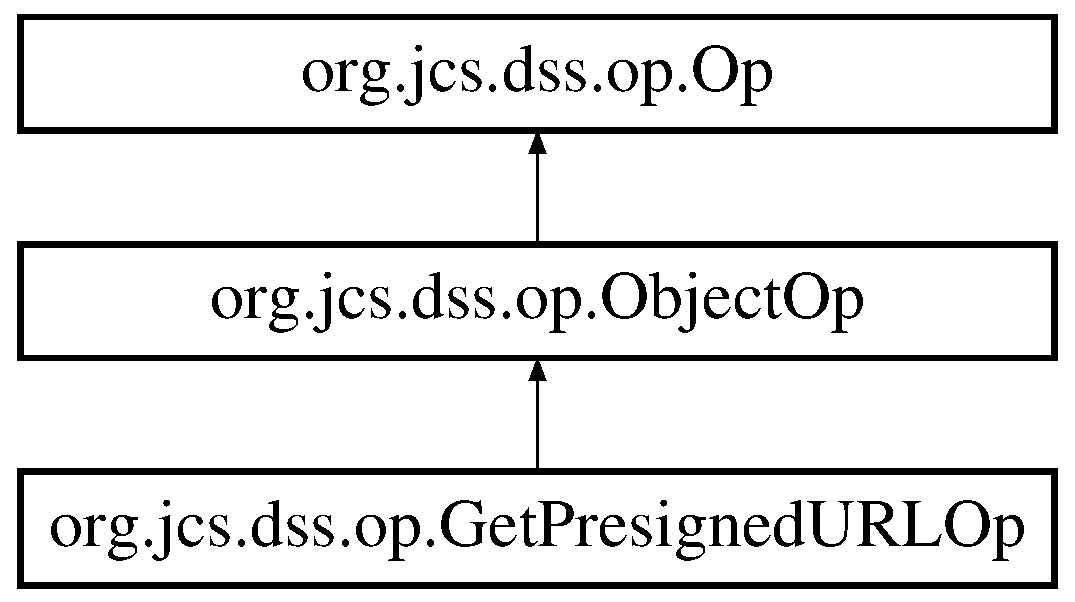
\includegraphics[height=3.000000cm]{classorg_1_1jcs_1_1dss_1_1op_1_1GetPresignedURLOp}
\end{center}
\end{figure}
\subsection*{Public Member Functions}
\begin{DoxyCompactItemize}
\item 
\hyperlink{classorg_1_1jcs_1_1dss_1_1op_1_1GetPresignedURLOp_a6e64e303788d28cfa3fb680eae98c761}{Get\+Presigned\+U\+R\+L\+Op} (Dss\+Connection conn, String bucket\+Name, String object\+Name, int Expiry)\hypertarget{classorg_1_1jcs_1_1dss_1_1op_1_1GetPresignedURLOp_a6e64e303788d28cfa3fb680eae98c761}{}\label{classorg_1_1jcs_1_1dss_1_1op_1_1GetPresignedURLOp_a6e64e303788d28cfa3fb680eae98c761}

\begin{DoxyCompactList}\small\item\em Constructors. \end{DoxyCompactList}\item 
U\+RL \hyperlink{classorg_1_1jcs_1_1dss_1_1op_1_1GetPresignedURLOp_a7a53d9a226d5f47838850d3f989635b2}{Execute} ()  throws Exception 
\item 
U\+RL \hyperlink{classorg_1_1jcs_1_1dss_1_1op_1_1GetPresignedURLOp_a5e66c5007ee4990fd4a1a9b345336b3b}{Make\+Request} ()  throws Exception 
\begin{DoxyCompactList}\small\item\em This method first gets signature, sets http\+Headers and returns pre-\/signed U\+RL. \end{DoxyCompactList}\end{DoxyCompactItemize}
\subsection*{Additional Inherited Members}


\subsection{Detailed Description}
Class to get presigned url. 

\subsection{Member Function Documentation}
\index{org\+::jcs\+::dss\+::op\+::\+Get\+Presigned\+U\+R\+L\+Op@{org\+::jcs\+::dss\+::op\+::\+Get\+Presigned\+U\+R\+L\+Op}!Execute@{Execute}}
\index{Execute@{Execute}!org\+::jcs\+::dss\+::op\+::\+Get\+Presigned\+U\+R\+L\+Op@{org\+::jcs\+::dss\+::op\+::\+Get\+Presigned\+U\+R\+L\+Op}}
\subsubsection[{\texorpdfstring{Execute()}{Execute()}}]{\setlength{\rightskip}{0pt plus 5cm}U\+RL org.\+jcs.\+dss.\+op.\+Get\+Presigned\+U\+R\+L\+Op.\+Execute (
\begin{DoxyParamCaption}
{}
\end{DoxyParamCaption}
) throws Exception\hspace{0.3cm}{\ttfamily [inline]}}\hypertarget{classorg_1_1jcs_1_1dss_1_1op_1_1GetPresignedURLOp_a7a53d9a226d5f47838850d3f989635b2}{}\label{classorg_1_1jcs_1_1dss_1_1op_1_1GetPresignedURLOp_a7a53d9a226d5f47838850d3f989635b2}
\begin{DoxyReturn}{Returns}
U\+RL \+: Presigned U\+RL 
\end{DoxyReturn}

\begin{DoxyExceptions}{Exceptions}
{\em Exception} & \\
\hline
\end{DoxyExceptions}
\index{org\+::jcs\+::dss\+::op\+::\+Get\+Presigned\+U\+R\+L\+Op@{org\+::jcs\+::dss\+::op\+::\+Get\+Presigned\+U\+R\+L\+Op}!Make\+Request@{Make\+Request}}
\index{Make\+Request@{Make\+Request}!org\+::jcs\+::dss\+::op\+::\+Get\+Presigned\+U\+R\+L\+Op@{org\+::jcs\+::dss\+::op\+::\+Get\+Presigned\+U\+R\+L\+Op}}
\subsubsection[{\texorpdfstring{Make\+Request()}{MakeRequest()}}]{\setlength{\rightskip}{0pt plus 5cm}U\+RL org.\+jcs.\+dss.\+op.\+Get\+Presigned\+U\+R\+L\+Op.\+Make\+Request (
\begin{DoxyParamCaption}
{}
\end{DoxyParamCaption}
) throws Exception\hspace{0.3cm}{\ttfamily [inline]}}\hypertarget{classorg_1_1jcs_1_1dss_1_1op_1_1GetPresignedURLOp_a5e66c5007ee4990fd4a1a9b345336b3b}{}\label{classorg_1_1jcs_1_1dss_1_1op_1_1GetPresignedURLOp_a5e66c5007ee4990fd4a1a9b345336b3b}


This method first gets signature, sets http\+Headers and returns pre-\/signed U\+RL. 

\begin{DoxyReturn}{Returns}
U\+RL \+: Presigned U\+RL 
\end{DoxyReturn}
Creating object of Dss\+Auth to get signature 

The documentation for this class was generated from the following file\+:\begin{DoxyCompactItemize}
\item 
Get\+Presigned\+U\+R\+L\+Op.\+java\end{DoxyCompactItemize}

\hypertarget{classorg_1_1jcs_1_1dss_1_1op_1_1HeadBucketOp}{}\section{org.\+jcs.\+dss.\+op.\+Head\+Bucket\+Op Class Reference}
\label{classorg_1_1jcs_1_1dss_1_1op_1_1HeadBucketOp}\index{org.\+jcs.\+dss.\+op.\+Head\+Bucket\+Op@{org.\+jcs.\+dss.\+op.\+Head\+Bucket\+Op}}


Class to execute head bucket A\+PI.  


Inheritance diagram for org.\+jcs.\+dss.\+op.\+Head\+Bucket\+Op\+:\begin{figure}[H]
\begin{center}
\leavevmode
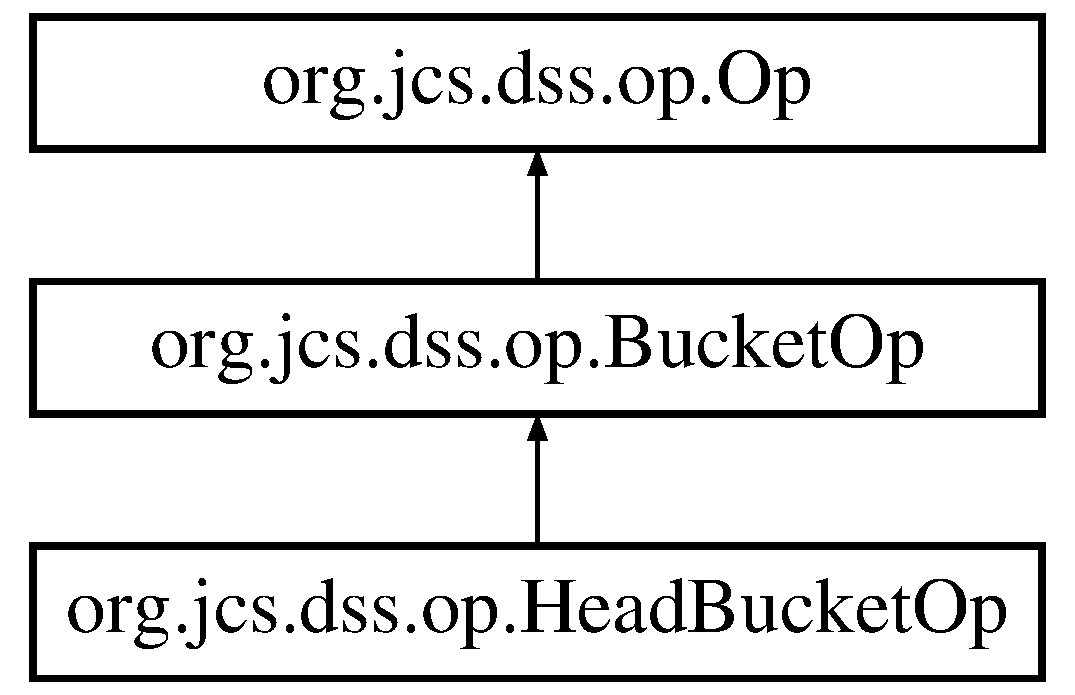
\includegraphics[height=3.000000cm]{classorg_1_1jcs_1_1dss_1_1op_1_1HeadBucketOp}
\end{center}
\end{figure}
\subsection*{Public Member Functions}
\begin{DoxyCompactItemize}
\item 
\hyperlink{classorg_1_1jcs_1_1dss_1_1op_1_1HeadBucketOp_aecd0d24ca7cba476670ec546582e2f99}{Head\+Bucket\+Op} (Dss\+Connection conn, String bucket\+Name)\hypertarget{classorg_1_1jcs_1_1dss_1_1op_1_1HeadBucketOp_aecd0d24ca7cba476670ec546582e2f99}{}\label{classorg_1_1jcs_1_1dss_1_1op_1_1HeadBucketOp_aecd0d24ca7cba476670ec546582e2f99}

\begin{DoxyCompactList}\small\item\em Constructors. \end{DoxyCompactList}\end{DoxyCompactItemize}
\subsection*{Additional Inherited Members}


\subsection{Detailed Description}
Class to execute head bucket A\+PI. 

The documentation for this class was generated from the following file\+:\begin{DoxyCompactItemize}
\item 
Head\+Bucket\+Op.\+java\end{DoxyCompactItemize}

\hypertarget{classorg_1_1jcs_1_1dss_1_1op_1_1HeadObjectOp}{}\section{org.\+jcs.\+dss.\+op.\+Head\+Object\+Op Class Reference}
\label{classorg_1_1jcs_1_1dss_1_1op_1_1HeadObjectOp}\index{org.\+jcs.\+dss.\+op.\+Head\+Object\+Op@{org.\+jcs.\+dss.\+op.\+Head\+Object\+Op}}


Class to execute head object A\+PI.  


Inheritance diagram for org.\+jcs.\+dss.\+op.\+Head\+Object\+Op\+:\begin{figure}[H]
\begin{center}
\leavevmode
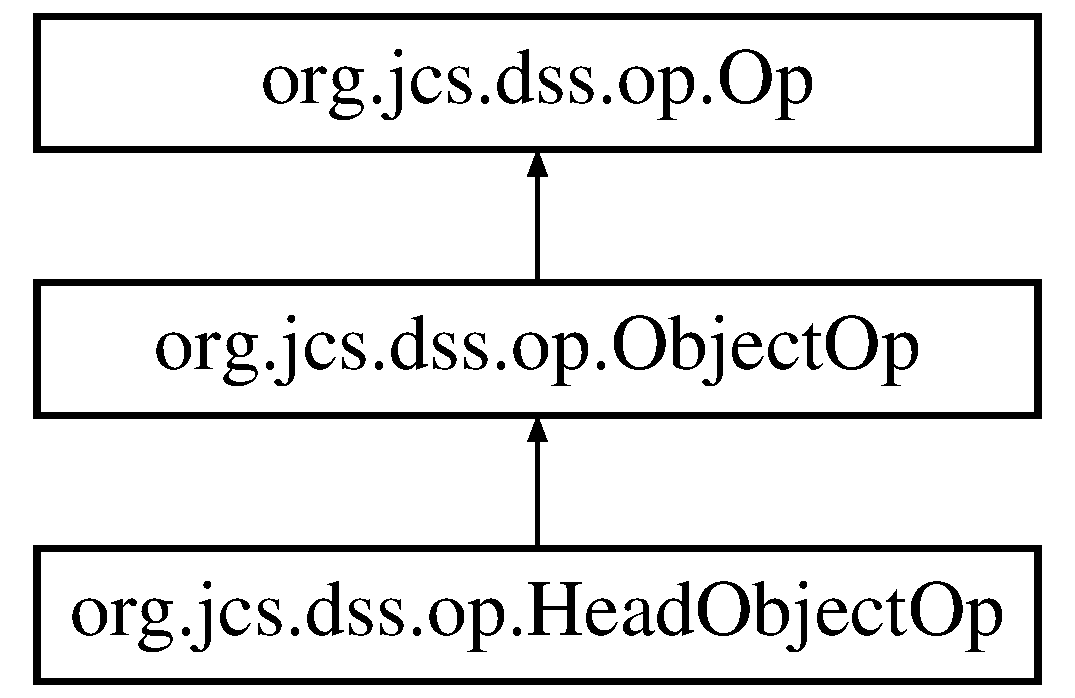
\includegraphics[height=3.000000cm]{classorg_1_1jcs_1_1dss_1_1op_1_1HeadObjectOp}
\end{center}
\end{figure}
\subsection*{Public Member Functions}
\begin{DoxyCompactItemize}
\item 
\hyperlink{classorg_1_1jcs_1_1dss_1_1op_1_1HeadObjectOp_a6fe2525bad4cb66ba7a8db109ea5d220}{Head\+Object\+Op} (Dss\+Connection conn, String bucket\+Name, String object\+Name)\hypertarget{classorg_1_1jcs_1_1dss_1_1op_1_1HeadObjectOp_a6fe2525bad4cb66ba7a8db109ea5d220}{}\label{classorg_1_1jcs_1_1dss_1_1op_1_1HeadObjectOp_a6fe2525bad4cb66ba7a8db109ea5d220}

\begin{DoxyCompactList}\small\item\em Constructors. \end{DoxyCompactList}\end{DoxyCompactItemize}
\subsection*{Additional Inherited Members}


\subsection{Detailed Description}
Class to execute head object A\+PI. 

The documentation for this class was generated from the following file\+:\begin{DoxyCompactItemize}
\item 
Head\+Object\+Op.\+java\end{DoxyCompactItemize}

\hypertarget{classorg_1_1jcs_1_1dss_1_1op_1_1InitMPUploadOp}{}\section{org.\+jcs.\+dss.\+op.\+Init\+M\+P\+Upload\+Op Class Reference}
\label{classorg_1_1jcs_1_1dss_1_1op_1_1InitMPUploadOp}\index{org.\+jcs.\+dss.\+op.\+Init\+M\+P\+Upload\+Op@{org.\+jcs.\+dss.\+op.\+Init\+M\+P\+Upload\+Op}}


Class to Initiate Multi\+Part Upload.  


Inheritance diagram for org.\+jcs.\+dss.\+op.\+Init\+M\+P\+Upload\+Op\+:\begin{figure}[H]
\begin{center}
\leavevmode
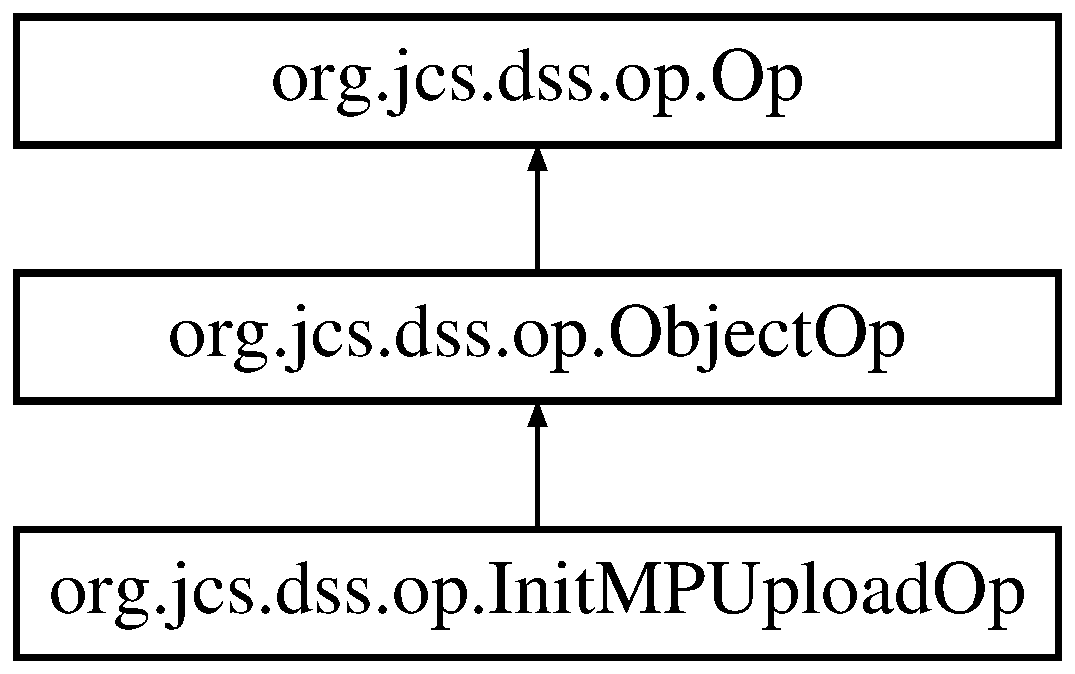
\includegraphics[height=3.000000cm]{classorg_1_1jcs_1_1dss_1_1op_1_1InitMPUploadOp}
\end{center}
\end{figure}
\subsection*{Public Member Functions}
\begin{DoxyCompactItemize}
\item 
\hyperlink{classorg_1_1jcs_1_1dss_1_1op_1_1InitMPUploadOp_a33e5403cd929ba5cf46987e1dc6858c0}{Init\+M\+P\+Upload\+Op} (Dss\+Connection conn, String bucket\+Name, String object\+Name)\hypertarget{classorg_1_1jcs_1_1dss_1_1op_1_1InitMPUploadOp_a33e5403cd929ba5cf46987e1dc6858c0}{}\label{classorg_1_1jcs_1_1dss_1_1op_1_1InitMPUploadOp_a33e5403cd929ba5cf46987e1dc6858c0}

\begin{DoxyCompactList}\small\item\em Constructors. \end{DoxyCompactList}\item 
Object \hyperlink{classorg_1_1jcs_1_1dss_1_1op_1_1InitMPUploadOp_a6ecc510bdcc5f8301f42865f7a83d4f9}{process\+Result} (Object resp)  throws I\+O\+Exception
\begin{DoxyCompactList}\small\item\em This method extracts information such as key, Upload\+Id etc from Input\+Stream got from Server. \end{DoxyCompactList}\end{DoxyCompactItemize}
\subsection*{Additional Inherited Members}


\subsection{Detailed Description}
Class to Initiate Multi\+Part Upload. 

\subsection{Member Function Documentation}
\index{org\+::jcs\+::dss\+::op\+::\+Init\+M\+P\+Upload\+Op@{org\+::jcs\+::dss\+::op\+::\+Init\+M\+P\+Upload\+Op}!process\+Result@{process\+Result}}
\index{process\+Result@{process\+Result}!org\+::jcs\+::dss\+::op\+::\+Init\+M\+P\+Upload\+Op@{org\+::jcs\+::dss\+::op\+::\+Init\+M\+P\+Upload\+Op}}
\subsubsection[{\texorpdfstring{process\+Result(\+Object resp)}{processResult(Object resp)}}]{\setlength{\rightskip}{0pt plus 5cm}Object org.\+jcs.\+dss.\+op.\+Init\+M\+P\+Upload\+Op.\+process\+Result (
\begin{DoxyParamCaption}
\item[{Object}]{resp}
\end{DoxyParamCaption}
) throws I\+O\+Exception\hspace{0.3cm}{\ttfamily [inline]}}\hypertarget{classorg_1_1jcs_1_1dss_1_1op_1_1InitMPUploadOp_a6ecc510bdcc5f8301f42865f7a83d4f9}{}\label{classorg_1_1jcs_1_1dss_1_1op_1_1InitMPUploadOp_a6ecc510bdcc5f8301f42865f7a83d4f9}


This method extracts information such as key, Upload\+Id etc from Input\+Stream got from Server. 


\begin{DoxyParams}{Parameters}
{\em Response} & \+: Response message got from Request.\+put() \\
\hline
\end{DoxyParams}
\begin{DoxyReturn}{Returns}
Initiate\+Multipart\+Upload\+Result \+: A class that contains all the information about a initiated Multi\+Part upload 
\end{DoxyReturn}

\begin{DoxyExceptions}{Exceptions}
{\em I\+O\+Exception} & \\
\hline
\end{DoxyExceptions}


The documentation for this class was generated from the following file\+:\begin{DoxyCompactItemize}
\item 
Init\+M\+P\+Upload\+Op.\+java\end{DoxyCompactItemize}

\hypertarget{classorg_1_1jcs_1_1dss_1_1op_1_1ListBucketsOp}{}\section{org.\+jcs.\+dss.\+op.\+List\+Buckets\+Op Class Reference}
\label{classorg_1_1jcs_1_1dss_1_1op_1_1ListBucketsOp}\index{org.\+jcs.\+dss.\+op.\+List\+Buckets\+Op@{org.\+jcs.\+dss.\+op.\+List\+Buckets\+Op}}


Class to get List of all Buckets associated with the this account.  


Inheritance diagram for org.\+jcs.\+dss.\+op.\+List\+Buckets\+Op\+:\begin{figure}[H]
\begin{center}
\leavevmode
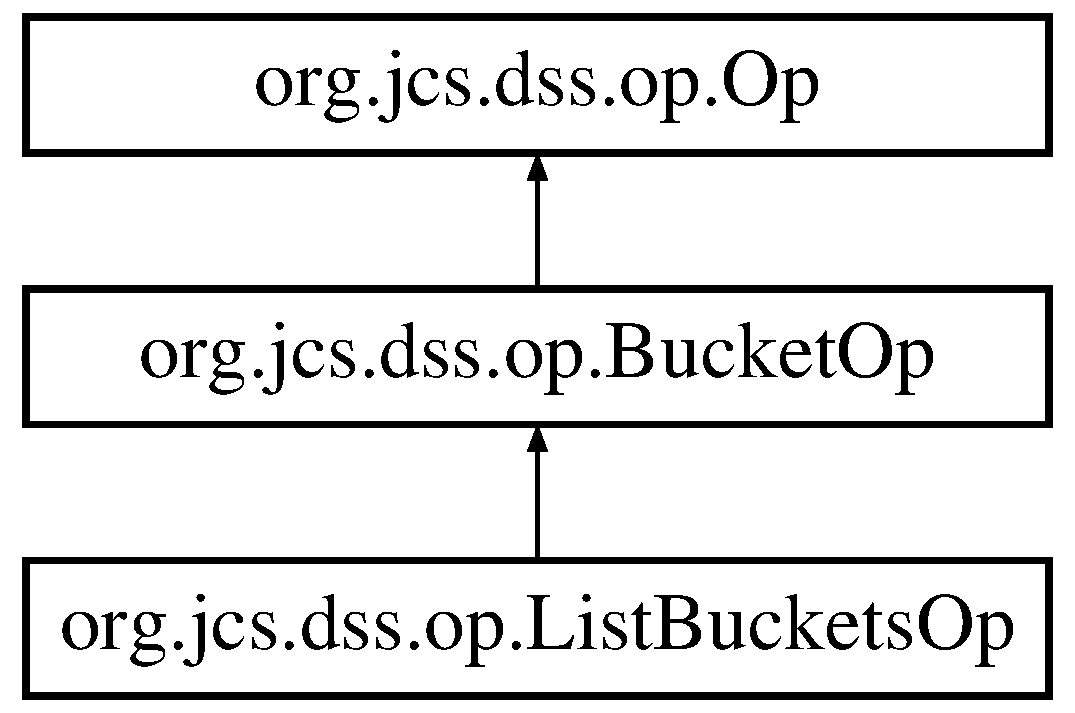
\includegraphics[height=3.000000cm]{classorg_1_1jcs_1_1dss_1_1op_1_1ListBucketsOp}
\end{center}
\end{figure}
\subsection*{Public Member Functions}
\begin{DoxyCompactItemize}
\item 
\hyperlink{classorg_1_1jcs_1_1dss_1_1op_1_1ListBucketsOp_a753f4dede03a1bdf70af02b6353a7f24}{List\+Buckets\+Op} (Dss\+Connection conn)\hypertarget{classorg_1_1jcs_1_1dss_1_1op_1_1ListBucketsOp_a753f4dede03a1bdf70af02b6353a7f24}{}\label{classorg_1_1jcs_1_1dss_1_1op_1_1ListBucketsOp_a753f4dede03a1bdf70af02b6353a7f24}

\begin{DoxyCompactList}\small\item\em Constructors. \end{DoxyCompactList}\item 
Object \hyperlink{classorg_1_1jcs_1_1dss_1_1op_1_1ListBucketsOp_abe4f8f93c6a8da17a4e56915de1445f7}{process\+Result} (Object resp)  throws I\+O\+Exception
\begin{DoxyCompactList}\small\item\em This method extracts information such as Owner, Bucket name and creation date from Input\+Stream got from Server. \end{DoxyCompactList}\end{DoxyCompactItemize}
\subsection*{Additional Inherited Members}


\subsection{Detailed Description}
Class to get List of all Buckets associated with the this account. 

\subsection{Member Function Documentation}
\index{org\+::jcs\+::dss\+::op\+::\+List\+Buckets\+Op@{org\+::jcs\+::dss\+::op\+::\+List\+Buckets\+Op}!process\+Result@{process\+Result}}
\index{process\+Result@{process\+Result}!org\+::jcs\+::dss\+::op\+::\+List\+Buckets\+Op@{org\+::jcs\+::dss\+::op\+::\+List\+Buckets\+Op}}
\subsubsection[{\texorpdfstring{process\+Result(\+Object resp)}{processResult(Object resp)}}]{\setlength{\rightskip}{0pt plus 5cm}Object org.\+jcs.\+dss.\+op.\+List\+Buckets\+Op.\+process\+Result (
\begin{DoxyParamCaption}
\item[{Object}]{resp}
\end{DoxyParamCaption}
) throws I\+O\+Exception\hspace{0.3cm}{\ttfamily [inline]}}\hypertarget{classorg_1_1jcs_1_1dss_1_1op_1_1ListBucketsOp_abe4f8f93c6a8da17a4e56915de1445f7}{}\label{classorg_1_1jcs_1_1dss_1_1op_1_1ListBucketsOp_abe4f8f93c6a8da17a4e56915de1445f7}


This method extracts information such as Owner, Bucket name and creation date from Input\+Stream got from Server. 


\begin{DoxyParams}{Parameters}
{\em Response} & \+: Response message got from Request.\+request() \\
\hline
\end{DoxyParams}
\begin{DoxyReturn}{Returns}
List$<$\+Bucket$>$ \+: List of all D\+SS buckets associated with this account 
\end{DoxyReturn}

\begin{DoxyExceptions}{Exceptions}
{\em I\+O\+Exception} & \\
\hline
\end{DoxyExceptions}


The documentation for this class was generated from the following file\+:\begin{DoxyCompactItemize}
\item 
List\+Buckets\+Op.\+java\end{DoxyCompactItemize}

\hypertarget{classorg_1_1jcs_1_1dss_1_1op_1_1ListMPUploadsOp}{}\section{org.\+jcs.\+dss.\+op.\+List\+M\+P\+Uploads\+Op Class Reference}
\label{classorg_1_1jcs_1_1dss_1_1op_1_1ListMPUploadsOp}\index{org.\+jcs.\+dss.\+op.\+List\+M\+P\+Uploads\+Op@{org.\+jcs.\+dss.\+op.\+List\+M\+P\+Uploads\+Op}}


Class to list all the on-\/going Multi\+Part uploads associated with the requested bucket.  


Inheritance diagram for org.\+jcs.\+dss.\+op.\+List\+M\+P\+Uploads\+Op\+:\begin{figure}[H]
\begin{center}
\leavevmode
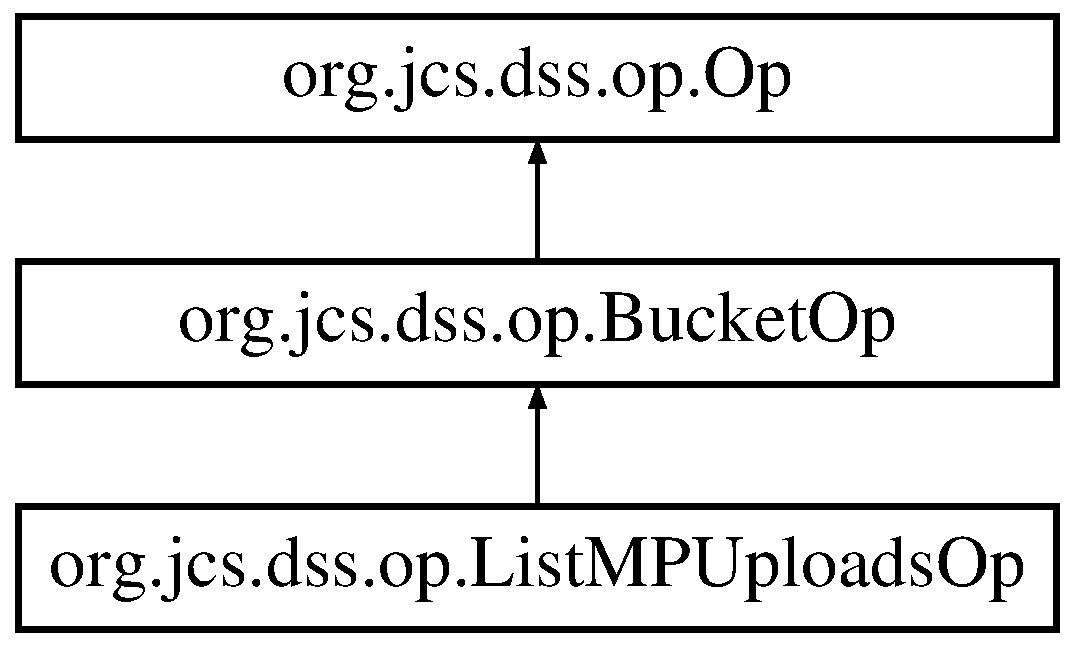
\includegraphics[height=3.000000cm]{classorg_1_1jcs_1_1dss_1_1op_1_1ListMPUploadsOp}
\end{center}
\end{figure}
\subsection*{Public Member Functions}
\begin{DoxyCompactItemize}
\item 
\hyperlink{classorg_1_1jcs_1_1dss_1_1op_1_1ListMPUploadsOp_a860cbabfda88cbbeeac14d14bb956d65}{List\+M\+P\+Uploads\+Op} (Dss\+Connection conn, String bucket\+Name)\hypertarget{classorg_1_1jcs_1_1dss_1_1op_1_1ListMPUploadsOp_a860cbabfda88cbbeeac14d14bb956d65}{}\label{classorg_1_1jcs_1_1dss_1_1op_1_1ListMPUploadsOp_a860cbabfda88cbbeeac14d14bb956d65}

\begin{DoxyCompactList}\small\item\em Constructors. \end{DoxyCompactList}\item 
Object \hyperlink{classorg_1_1jcs_1_1dss_1_1op_1_1ListMPUploadsOp_aa2e55e3ae139072f10b2777a1f879643}{process\+Result} (Object resp)  throws I\+O\+Exception
\begin{DoxyCompactList}\small\item\em This method extracts information such as key, E\+Tag etc from Input\+Stream got from Server. \end{DoxyCompactList}\end{DoxyCompactItemize}
\subsection*{Additional Inherited Members}


\subsection{Detailed Description}
Class to list all the on-\/going Multi\+Part uploads associated with the requested bucket. 

\subsection{Member Function Documentation}
\index{org\+::jcs\+::dss\+::op\+::\+List\+M\+P\+Uploads\+Op@{org\+::jcs\+::dss\+::op\+::\+List\+M\+P\+Uploads\+Op}!process\+Result@{process\+Result}}
\index{process\+Result@{process\+Result}!org\+::jcs\+::dss\+::op\+::\+List\+M\+P\+Uploads\+Op@{org\+::jcs\+::dss\+::op\+::\+List\+M\+P\+Uploads\+Op}}
\subsubsection[{\texorpdfstring{process\+Result(\+Object resp)}{processResult(Object resp)}}]{\setlength{\rightskip}{0pt plus 5cm}Object org.\+jcs.\+dss.\+op.\+List\+M\+P\+Uploads\+Op.\+process\+Result (
\begin{DoxyParamCaption}
\item[{Object}]{resp}
\end{DoxyParamCaption}
) throws I\+O\+Exception\hspace{0.3cm}{\ttfamily [inline]}}\hypertarget{classorg_1_1jcs_1_1dss_1_1op_1_1ListMPUploadsOp_aa2e55e3ae139072f10b2777a1f879643}{}\label{classorg_1_1jcs_1_1dss_1_1op_1_1ListMPUploadsOp_aa2e55e3ae139072f10b2777a1f879643}


This method extracts information such as key, E\+Tag etc from Input\+Stream got from Server. 


\begin{DoxyParams}{Parameters}
{\em Response} & \+: Response message got from Request.\+request() \\
\hline
\end{DoxyParams}
\begin{DoxyReturn}{Returns}
Complete\+Multipart\+Upload\+Result \+: A class that contains all the information about a successful uploaded object 
\end{DoxyReturn}

\begin{DoxyExceptions}{Exceptions}
{\em I\+O\+Exception} & \\
\hline
\end{DoxyExceptions}


The documentation for this class was generated from the following file\+:\begin{DoxyCompactItemize}
\item 
List\+M\+P\+Uploads\+Op.\+java\end{DoxyCompactItemize}

\hypertarget{classorg_1_1jcs_1_1dss_1_1op_1_1ListObjectsOp}{}\section{org.\+jcs.\+dss.\+op.\+List\+Objects\+Op Class Reference}
\label{classorg_1_1jcs_1_1dss_1_1op_1_1ListObjectsOp}\index{org.\+jcs.\+dss.\+op.\+List\+Objects\+Op@{org.\+jcs.\+dss.\+op.\+List\+Objects\+Op}}


Class to get List of all Objects associated with the requested bucket.  


Inheritance diagram for org.\+jcs.\+dss.\+op.\+List\+Objects\+Op\+:\begin{figure}[H]
\begin{center}
\leavevmode
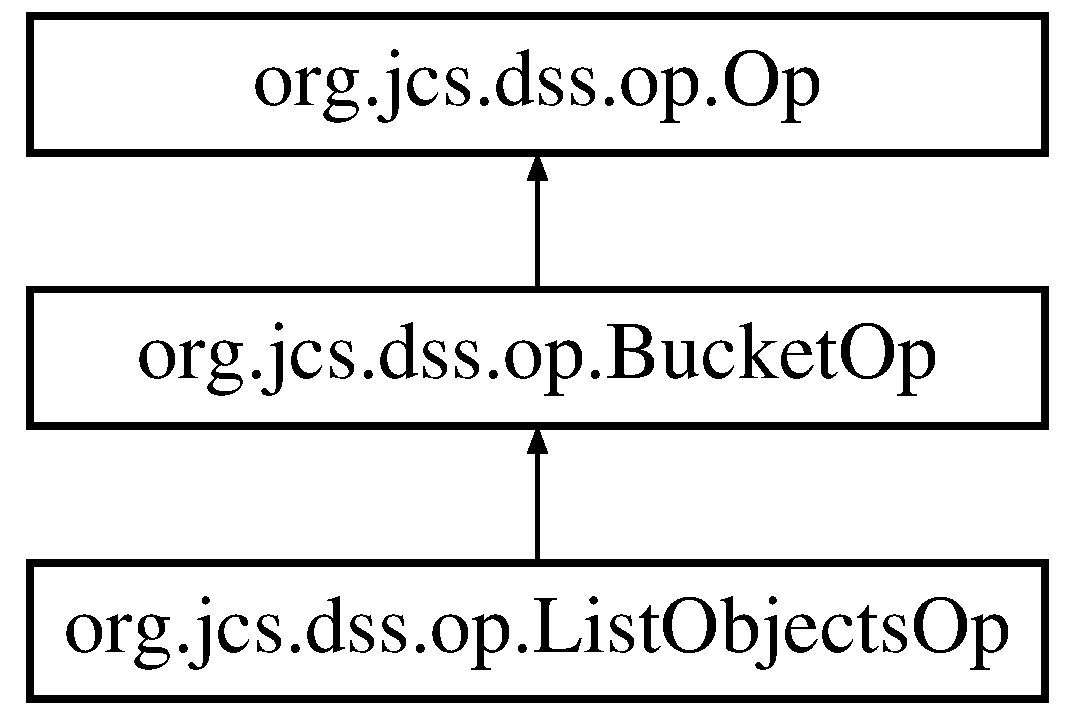
\includegraphics[height=3.000000cm]{classorg_1_1jcs_1_1dss_1_1op_1_1ListObjectsOp}
\end{center}
\end{figure}
\subsection*{Public Member Functions}
\begin{DoxyCompactItemize}
\item 
\hyperlink{classorg_1_1jcs_1_1dss_1_1op_1_1ListObjectsOp_ae1f56ad3eedea91db238576334238dc6}{List\+Objects\+Op} (Dss\+Connection conn, String bucket\+Name)\hypertarget{classorg_1_1jcs_1_1dss_1_1op_1_1ListObjectsOp_ae1f56ad3eedea91db238576334238dc6}{}\label{classorg_1_1jcs_1_1dss_1_1op_1_1ListObjectsOp_ae1f56ad3eedea91db238576334238dc6}

\begin{DoxyCompactList}\small\item\em Constructors. \end{DoxyCompactList}\item 
Object \hyperlink{classorg_1_1jcs_1_1dss_1_1op_1_1ListObjectsOp_a78c2014b20163ca5cd5dfd47c4b181f3}{process\+Result} (Object resp)  throws I\+O\+Exception
\begin{DoxyCompactList}\small\item\em This method extracts information such as Size, Key etc about each object from Input\+Stream got from Server. \end{DoxyCompactList}\end{DoxyCompactItemize}
\subsection*{Additional Inherited Members}


\subsection{Detailed Description}
Class to get List of all Objects associated with the requested bucket. 

\subsection{Member Function Documentation}
\index{org\+::jcs\+::dss\+::op\+::\+List\+Objects\+Op@{org\+::jcs\+::dss\+::op\+::\+List\+Objects\+Op}!process\+Result@{process\+Result}}
\index{process\+Result@{process\+Result}!org\+::jcs\+::dss\+::op\+::\+List\+Objects\+Op@{org\+::jcs\+::dss\+::op\+::\+List\+Objects\+Op}}
\subsubsection[{\texorpdfstring{process\+Result(\+Object resp)}{processResult(Object resp)}}]{\setlength{\rightskip}{0pt plus 5cm}Object org.\+jcs.\+dss.\+op.\+List\+Objects\+Op.\+process\+Result (
\begin{DoxyParamCaption}
\item[{Object}]{resp}
\end{DoxyParamCaption}
) throws I\+O\+Exception\hspace{0.3cm}{\ttfamily [inline]}}\hypertarget{classorg_1_1jcs_1_1dss_1_1op_1_1ListObjectsOp_a78c2014b20163ca5cd5dfd47c4b181f3}{}\label{classorg_1_1jcs_1_1dss_1_1op_1_1ListObjectsOp_a78c2014b20163ca5cd5dfd47c4b181f3}


This method extracts information such as Size, Key etc about each object from Input\+Stream got from Server. 


\begin{DoxyParams}{Parameters}
{\em Response} & \+: Response message got from Request.\+request() \\
\hline
\end{DoxyParams}
\begin{DoxyReturn}{Returns}
List$<$\+Dss\+Object$>$ \+: List of all D\+SS Objects associated with the requested bucket 
\end{DoxyReturn}

\begin{DoxyExceptions}{Exceptions}
{\em I\+O\+Exception} & \\
\hline
\end{DoxyExceptions}


The documentation for this class was generated from the following file\+:\begin{DoxyCompactItemize}
\item 
List\+Objects\+Op.\+java\end{DoxyCompactItemize}

\hypertarget{classorg_1_1jcs_1_1dss_1_1op_1_1ListPartOp}{}\section{org.\+jcs.\+dss.\+op.\+List\+Part\+Op Class Reference}
\label{classorg_1_1jcs_1_1dss_1_1op_1_1ListPartOp}\index{org.\+jcs.\+dss.\+op.\+List\+Part\+Op@{org.\+jcs.\+dss.\+op.\+List\+Part\+Op}}


Class to execute List Part A\+PI.  


Inheritance diagram for org.\+jcs.\+dss.\+op.\+List\+Part\+Op\+:\begin{figure}[H]
\begin{center}
\leavevmode
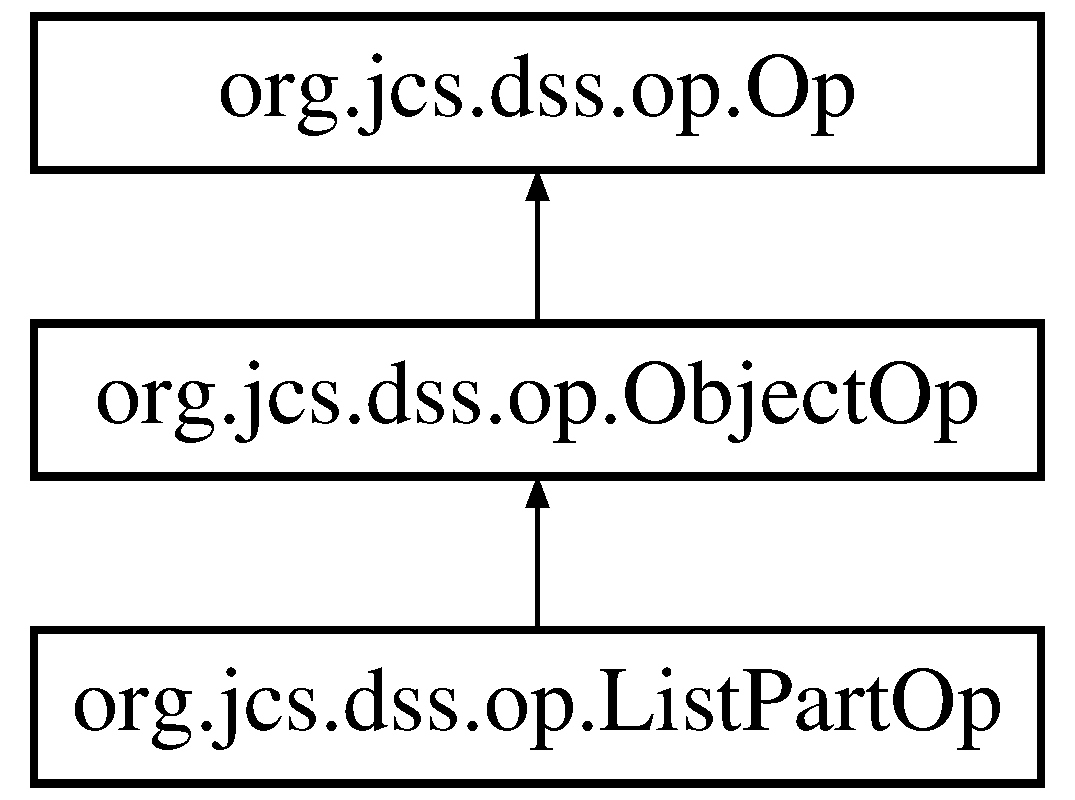
\includegraphics[height=3.000000cm]{classorg_1_1jcs_1_1dss_1_1op_1_1ListPartOp}
\end{center}
\end{figure}
\subsection*{Public Member Functions}
\begin{DoxyCompactItemize}
\item 
\hyperlink{classorg_1_1jcs_1_1dss_1_1op_1_1ListPartOp_a3783f9f4cfd10805e57756f359a734fe}{List\+Part\+Op} (Dss\+Connection conn, String bucket\+Name, String object\+Name, String upload\+Id)\hypertarget{classorg_1_1jcs_1_1dss_1_1op_1_1ListPartOp_a3783f9f4cfd10805e57756f359a734fe}{}\label{classorg_1_1jcs_1_1dss_1_1op_1_1ListPartOp_a3783f9f4cfd10805e57756f359a734fe}

\begin{DoxyCompactList}\small\item\em Constructors. \end{DoxyCompactList}\item 
Object \hyperlink{classorg_1_1jcs_1_1dss_1_1op_1_1ListPartOp_a2dc96679605e098dc2f7f37076cef252}{process\+Result} (Object resp)  throws I\+O\+Exception
\begin{DoxyCompactList}\small\item\em This method extracts information such as size,part number, E\+Tag etc from Input\+Stream got from Server. \end{DoxyCompactList}\end{DoxyCompactItemize}
\subsection*{Additional Inherited Members}


\subsection{Detailed Description}
Class to execute List Part A\+PI. 

\subsection{Member Function Documentation}
\index{org\+::jcs\+::dss\+::op\+::\+List\+Part\+Op@{org\+::jcs\+::dss\+::op\+::\+List\+Part\+Op}!process\+Result@{process\+Result}}
\index{process\+Result@{process\+Result}!org\+::jcs\+::dss\+::op\+::\+List\+Part\+Op@{org\+::jcs\+::dss\+::op\+::\+List\+Part\+Op}}
\subsubsection[{\texorpdfstring{process\+Result(\+Object resp)}{processResult(Object resp)}}]{\setlength{\rightskip}{0pt plus 5cm}Object org.\+jcs.\+dss.\+op.\+List\+Part\+Op.\+process\+Result (
\begin{DoxyParamCaption}
\item[{Object}]{resp}
\end{DoxyParamCaption}
) throws I\+O\+Exception\hspace{0.3cm}{\ttfamily [inline]}}\hypertarget{classorg_1_1jcs_1_1dss_1_1op_1_1ListPartOp_a2dc96679605e098dc2f7f37076cef252}{}\label{classorg_1_1jcs_1_1dss_1_1op_1_1ListPartOp_a2dc96679605e098dc2f7f37076cef252}


This method extracts information such as size,part number, E\+Tag etc from Input\+Stream got from Server. 


\begin{DoxyParams}{Parameters}
{\em Response} & \+: Response message got from Request.\+request() \\
\hline
\end{DoxyParams}
\begin{DoxyReturn}{Returns}
Part\+Listing \+: A class that contains all the information about each part associated with the requested key 
\end{DoxyReturn}

\begin{DoxyExceptions}{Exceptions}
{\em I\+O\+Exception} & \\
\hline
\end{DoxyExceptions}


The documentation for this class was generated from the following file\+:\begin{DoxyCompactItemize}
\item 
List\+Part\+Op.\+java\end{DoxyCompactItemize}

\hypertarget{classorg_1_1jcs_1_1dss_1_1op_1_1ObjectOp}{}\section{org.\+jcs.\+dss.\+op.\+Object\+Op Class Reference}
\label{classorg_1_1jcs_1_1dss_1_1op_1_1ObjectOp}\index{org.\+jcs.\+dss.\+op.\+Object\+Op@{org.\+jcs.\+dss.\+op.\+Object\+Op}}


Head Class for all operations related to objects.  


Inheritance diagram for org.\+jcs.\+dss.\+op.\+Object\+Op\+:\begin{figure}[H]
\begin{center}
\leavevmode
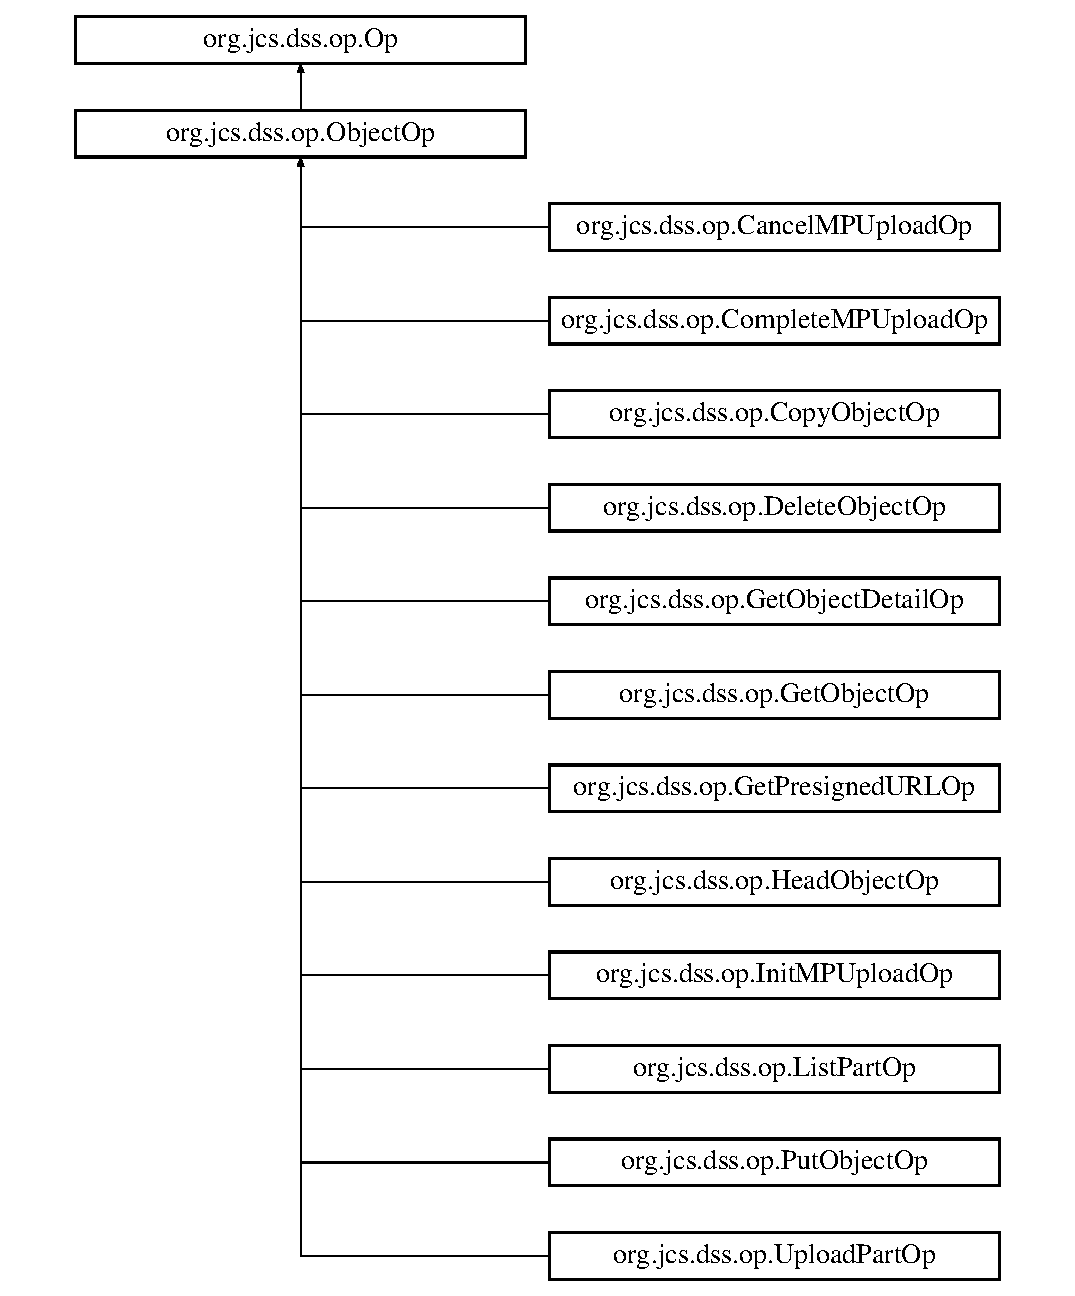
\includegraphics[height=12.000000cm]{classorg_1_1jcs_1_1dss_1_1op_1_1ObjectOp}
\end{center}
\end{figure}
\subsection*{Public Member Functions}
\begin{DoxyCompactItemize}
\item 
\hyperlink{classorg_1_1jcs_1_1dss_1_1op_1_1ObjectOp_a55f2bd7945ff68e1915eb6d9ea59ebd4}{Object\+Op} (Dss\+Connection conn, String bucket\+Name, String object\+Name)\hypertarget{classorg_1_1jcs_1_1dss_1_1op_1_1ObjectOp_a55f2bd7945ff68e1915eb6d9ea59ebd4}{}\label{classorg_1_1jcs_1_1dss_1_1op_1_1ObjectOp_a55f2bd7945ff68e1915eb6d9ea59ebd4}

\begin{DoxyCompactList}\small\item\em Constructors. \end{DoxyCompactList}\item 
Response \hyperlink{classorg_1_1jcs_1_1dss_1_1op_1_1ObjectOp_aefe80e395c9cb318f1a052e85362a520}{execute} ()  throws Exception 
\begin{DoxyCompactList}\small\item\em Executes the method requested by user. \end{DoxyCompactList}\item 
Object \hyperlink{classorg_1_1jcs_1_1dss_1_1op_1_1ObjectOp_a8d3b1fe1a3888deaa06e9f28e820d042}{process\+Result} (Object result)  throws I\+O\+Exception\hypertarget{classorg_1_1jcs_1_1dss_1_1op_1_1ObjectOp_a8d3b1fe1a3888deaa06e9f28e820d042}{}\label{classorg_1_1jcs_1_1dss_1_1op_1_1ObjectOp_a8d3b1fe1a3888deaa06e9f28e820d042}

\begin{DoxyCompactList}\small\item\em Processes the final result. \end{DoxyCompactList}\end{DoxyCompactItemize}
\subsection*{Additional Inherited Members}


\subsection{Detailed Description}
Head Class for all operations related to objects. 

\subsection{Member Function Documentation}
\index{org\+::jcs\+::dss\+::op\+::\+Object\+Op@{org\+::jcs\+::dss\+::op\+::\+Object\+Op}!execute@{execute}}
\index{execute@{execute}!org\+::jcs\+::dss\+::op\+::\+Object\+Op@{org\+::jcs\+::dss\+::op\+::\+Object\+Op}}
\subsubsection[{\texorpdfstring{execute()}{execute()}}]{\setlength{\rightskip}{0pt plus 5cm}Response org.\+jcs.\+dss.\+op.\+Object\+Op.\+execute (
\begin{DoxyParamCaption}
{}
\end{DoxyParamCaption}
) throws Exception\hspace{0.3cm}{\ttfamily [inline]}}\hypertarget{classorg_1_1jcs_1_1dss_1_1op_1_1ObjectOp_aefe80e395c9cb318f1a052e85362a520}{}\label{classorg_1_1jcs_1_1dss_1_1op_1_1ObjectOp_aefe80e395c9cb318f1a052e85362a520}


Executes the method requested by user. 

\begin{DoxyReturn}{Returns}
Response \+: Gets response object returned from \hyperlink{classorg_1_1jcs_1_1dss_1_1op_1_1Op_a8502896422a70d8e8f712b57490b1a91}{make\+Request()} 
\end{DoxyReturn}

\begin{DoxyExceptions}{Exceptions}
{\em Exception} & \\
\hline
\end{DoxyExceptions}


The documentation for this class was generated from the following file\+:\begin{DoxyCompactItemize}
\item 
Object\+Op.\+java\end{DoxyCompactItemize}

\hypertarget{classorg_1_1jcs_1_1dss_1_1op_1_1ObjectToXML}{}\section{org.\+jcs.\+dss.\+op.\+Object\+To\+X\+ML Class Reference}
\label{classorg_1_1jcs_1_1dss_1_1op_1_1ObjectToXML}\index{org.\+jcs.\+dss.\+op.\+Object\+To\+X\+ML@{org.\+jcs.\+dss.\+op.\+Object\+To\+X\+ML}}


Class to generate X\+ML string to be use in complete multi-\/part upload.  


\subsection*{Static Public Member Functions}
\begin{DoxyCompactItemize}
\item 
static String \hyperlink{classorg_1_1jcs_1_1dss_1_1op_1_1ObjectToXML_a890e47e18c5efb2db7401df3224ce8cf}{Genrate\+X\+ML} (List$<$ Upload\+Part\+Result $>$ Uploadpart)  throws J\+A\+X\+B\+Exception, I\+O\+Exception 
\begin{DoxyCompactList}\small\item\em Generation of string using J\+A\+XB marshalling. \end{DoxyCompactList}\end{DoxyCompactItemize}


\subsection{Detailed Description}
Class to generate X\+ML string to be use in complete multi-\/part upload. 

\subsection{Member Function Documentation}
\index{org\+::jcs\+::dss\+::op\+::\+Object\+To\+X\+ML@{org\+::jcs\+::dss\+::op\+::\+Object\+To\+X\+ML}!Genrate\+X\+ML@{Genrate\+X\+ML}}
\index{Genrate\+X\+ML@{Genrate\+X\+ML}!org\+::jcs\+::dss\+::op\+::\+Object\+To\+X\+ML@{org\+::jcs\+::dss\+::op\+::\+Object\+To\+X\+ML}}
\subsubsection[{\texorpdfstring{Genrate\+X\+M\+L(\+List$<$ Upload\+Part\+Result $>$ Uploadpart)}{GenrateXML(List< UploadPartResult > Uploadpart)}}]{\setlength{\rightskip}{0pt plus 5cm}static String org.\+jcs.\+dss.\+op.\+Object\+To\+X\+M\+L.\+Genrate\+X\+ML (
\begin{DoxyParamCaption}
\item[{List$<$ Upload\+Part\+Result $>$}]{Uploadpart}
\end{DoxyParamCaption}
) throws J\+A\+X\+B\+Exception, I\+O\+Exception\hspace{0.3cm}{\ttfamily [inline]}, {\ttfamily [static]}}\hypertarget{classorg_1_1jcs_1_1dss_1_1op_1_1ObjectToXML_a890e47e18c5efb2db7401df3224ce8cf}{}\label{classorg_1_1jcs_1_1dss_1_1op_1_1ObjectToXML_a890e47e18c5efb2db7401df3224ce8cf}


Generation of string using J\+A\+XB marshalling. 


\begin{DoxyParams}{Parameters}
{\em Uploadpart} & \+: List of E\+Tag and part number of all uploaded parts \\
\hline
\end{DoxyParams}
\begin{DoxyReturn}{Returns}
xml\+String \+: X\+ML String to be used in complete Multi-\/part upload 
\end{DoxyReturn}

\begin{DoxyExceptions}{Exceptions}
{\em J\+A\+X\+B\+Exception} & \\
\hline
{\em I\+O\+Exception} & \\
\hline
\end{DoxyExceptions}


The documentation for this class was generated from the following file\+:\begin{DoxyCompactItemize}
\item 
Object\+To\+X\+M\+L.\+java\end{DoxyCompactItemize}

\hypertarget{classorg_1_1jcs_1_1dss_1_1op_1_1Op}{}\section{org.\+jcs.\+dss.\+op.\+Op Class Reference}
\label{classorg_1_1jcs_1_1dss_1_1op_1_1Op}\index{org.\+jcs.\+dss.\+op.\+Op@{org.\+jcs.\+dss.\+op.\+Op}}


Head Class for all A\+PI operations.  


Inheritance diagram for org.\+jcs.\+dss.\+op.\+Op\+:\begin{figure}[H]
\begin{center}
\leavevmode
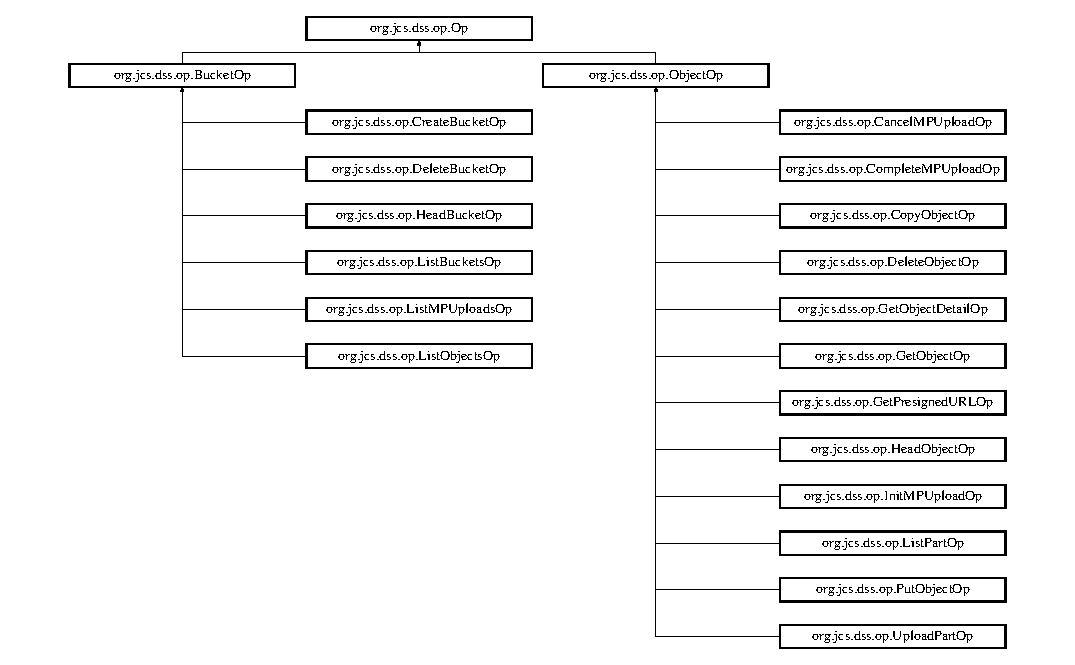
\includegraphics[height=8.484848cm]{classorg_1_1jcs_1_1dss_1_1op_1_1Op}
\end{center}
\end{figure}
\subsection*{Public Member Functions}
\begin{DoxyCompactItemize}
\item 
\hyperlink{classorg_1_1jcs_1_1dss_1_1op_1_1Op_a7a14d5b4d7eb1f579e9e6407ebcafe8e}{Op} (Dss\+Connection conn)\hypertarget{classorg_1_1jcs_1_1dss_1_1op_1_1Op_a7a14d5b4d7eb1f579e9e6407ebcafe8e}{}\label{classorg_1_1jcs_1_1dss_1_1op_1_1Op_a7a14d5b4d7eb1f579e9e6407ebcafe8e}

\begin{DoxyCompactList}\small\item\em Constructors. \end{DoxyCompactList}\item 
abstract Object \hyperlink{classorg_1_1jcs_1_1dss_1_1op_1_1Op_a8d268fda2eaa7be47a818427044189aa}{process\+Result} (Object result)  throws I\+O\+Exception\hypertarget{classorg_1_1jcs_1_1dss_1_1op_1_1Op_a8d268fda2eaa7be47a818427044189aa}{}\label{classorg_1_1jcs_1_1dss_1_1op_1_1Op_a8d268fda2eaa7be47a818427044189aa}

\begin{DoxyCompactList}\small\item\em Processes the final result. \end{DoxyCompactList}\item 
Response \hyperlink{classorg_1_1jcs_1_1dss_1_1op_1_1Op_a8502896422a70d8e8f712b57490b1a91}{make\+Request} ()  throws Exception 
\begin{DoxyCompactList}\small\item\em This method first gets signature, sets http\+Headers and then gets Response object. \end{DoxyCompactList}\end{DoxyCompactItemize}
\subsection*{Protected Attributes}
\begin{DoxyCompactItemize}
\item 
Dss\+Connection {\bfseries conn}\hypertarget{classorg_1_1jcs_1_1dss_1_1op_1_1Op_ab8a0bdf3a678af61b61af98ea5e26be7}{}\label{classorg_1_1jcs_1_1dss_1_1op_1_1Op_ab8a0bdf3a678af61b61af98ea5e26be7}

\item 
String {\bfseries http\+Method}\hypertarget{classorg_1_1jcs_1_1dss_1_1op_1_1Op_a34f4cea450ecada76563c4c9d533c339}{}\label{classorg_1_1jcs_1_1dss_1_1op_1_1Op_a34f4cea450ecada76563c4c9d533c339}

\item 
Map$<$ String, String $>$ {\bfseries http\+Headers}\hypertarget{classorg_1_1jcs_1_1dss_1_1op_1_1Op_a6db4bcd7b752123a1a85632000e86641}{}\label{classorg_1_1jcs_1_1dss_1_1op_1_1Op_a6db4bcd7b752123a1a85632000e86641}

\item 
String {\bfseries op\+Path}\hypertarget{classorg_1_1jcs_1_1dss_1_1op_1_1Op_a5f51c19ad6ad5d1b5b701409c824521c}{}\label{classorg_1_1jcs_1_1dss_1_1op_1_1Op_a5f51c19ad6ad5d1b5b701409c824521c}

\item 
String {\bfseries query\+Str}\hypertarget{classorg_1_1jcs_1_1dss_1_1op_1_1Op_a1705db02225f04d255eb4b5cbac99097}{}\label{classorg_1_1jcs_1_1dss_1_1op_1_1Op_a1705db02225f04d255eb4b5cbac99097}

\item 
String {\bfseries query\+Str\+For\+Signature}\hypertarget{classorg_1_1jcs_1_1dss_1_1op_1_1Op_aa6ea39ae1959b6d5cd939c48f22572a8}{}\label{classorg_1_1jcs_1_1dss_1_1op_1_1Op_aa6ea39ae1959b6d5cd939c48f22572a8}

\end{DoxyCompactItemize}


\subsection{Detailed Description}
Head Class for all A\+PI operations. 

\subsection{Member Function Documentation}
\index{org\+::jcs\+::dss\+::op\+::\+Op@{org\+::jcs\+::dss\+::op\+::\+Op}!make\+Request@{make\+Request}}
\index{make\+Request@{make\+Request}!org\+::jcs\+::dss\+::op\+::\+Op@{org\+::jcs\+::dss\+::op\+::\+Op}}
\subsubsection[{\texorpdfstring{make\+Request()}{makeRequest()}}]{\setlength{\rightskip}{0pt plus 5cm}Response org.\+jcs.\+dss.\+op.\+Op.\+make\+Request (
\begin{DoxyParamCaption}
{}
\end{DoxyParamCaption}
) throws Exception\hspace{0.3cm}{\ttfamily [inline]}}\hypertarget{classorg_1_1jcs_1_1dss_1_1op_1_1Op_a8502896422a70d8e8f712b57490b1a91}{}\label{classorg_1_1jcs_1_1dss_1_1op_1_1Op_a8502896422a70d8e8f712b57490b1a91}


This method first gets signature, sets http\+Headers and then gets Response object. 

\begin{DoxyReturn}{Returns}
Response \+: response object by calling request method under Request class 
\end{DoxyReturn}
Creating object of Dss\+Auth to get signature 

The documentation for this class was generated from the following file\+:\begin{DoxyCompactItemize}
\item 
Op.\+java\end{DoxyCompactItemize}

\hypertarget{classorg_1_1jcs_1_1dss_1_1op_1_1PartCreationForUploadPart}{}\section{org.\+jcs.\+dss.\+op.\+Part\+Creation\+For\+Upload\+Part Class Reference}
\label{classorg_1_1jcs_1_1dss_1_1op_1_1PartCreationForUploadPart}\index{org.\+jcs.\+dss.\+op.\+Part\+Creation\+For\+Upload\+Part@{org.\+jcs.\+dss.\+op.\+Part\+Creation\+For\+Upload\+Part}}


Class to break file into small parts of size requested by users to execute Upload\+Part A\+PI.  


\subsection*{Public Member Functions}
\begin{DoxyCompactItemize}
\item 
\hyperlink{classorg_1_1jcs_1_1dss_1_1op_1_1PartCreationForUploadPart_a4501ffcdcf569756434cb1edfb5e0679}{Part\+Creation\+For\+Upload\+Part} (Dss\+Connection conn, String bucket\+Name, String object\+Name, String upload\+Id, String file\+Path, int part\+Size)\hypertarget{classorg_1_1jcs_1_1dss_1_1op_1_1PartCreationForUploadPart_a4501ffcdcf569756434cb1edfb5e0679}{}\label{classorg_1_1jcs_1_1dss_1_1op_1_1PartCreationForUploadPart_a4501ffcdcf569756434cb1edfb5e0679}

\begin{DoxyCompactList}\small\item\em Constructors. \end{DoxyCompactList}\item 
List$<$ Upload\+Part\+Result $>$ \hyperlink{classorg_1_1jcs_1_1dss_1_1op_1_1PartCreationForUploadPart_aa57ac8879eb545556bf99f7456820461}{create\+Part} ()  throws Exception
\begin{DoxyCompactList}\small\item\em This method breaks file into smaller parts and creates its Input\+Stream and send to to \hyperlink{classorg_1_1jcs_1_1dss_1_1op_1_1UploadPartOp}{Upload\+Part\+Op} class to upload it on server and further extracts E\+Tag and part number corresponding to each part. \end{DoxyCompactList}\end{DoxyCompactItemize}


\subsection{Detailed Description}
Class to break file into small parts of size requested by users to execute Upload\+Part A\+PI. 

\subsection{Member Function Documentation}
\index{org\+::jcs\+::dss\+::op\+::\+Part\+Creation\+For\+Upload\+Part@{org\+::jcs\+::dss\+::op\+::\+Part\+Creation\+For\+Upload\+Part}!create\+Part@{create\+Part}}
\index{create\+Part@{create\+Part}!org\+::jcs\+::dss\+::op\+::\+Part\+Creation\+For\+Upload\+Part@{org\+::jcs\+::dss\+::op\+::\+Part\+Creation\+For\+Upload\+Part}}
\subsubsection[{\texorpdfstring{create\+Part()}{createPart()}}]{\setlength{\rightskip}{0pt plus 5cm}List$<$Upload\+Part\+Result$>$ org.\+jcs.\+dss.\+op.\+Part\+Creation\+For\+Upload\+Part.\+create\+Part (
\begin{DoxyParamCaption}
{}
\end{DoxyParamCaption}
) throws Exception\hspace{0.3cm}{\ttfamily [inline]}}\hypertarget{classorg_1_1jcs_1_1dss_1_1op_1_1PartCreationForUploadPart_aa57ac8879eb545556bf99f7456820461}{}\label{classorg_1_1jcs_1_1dss_1_1op_1_1PartCreationForUploadPart_aa57ac8879eb545556bf99f7456820461}


This method breaks file into smaller parts and creates its Input\+Stream and send to to \hyperlink{classorg_1_1jcs_1_1dss_1_1op_1_1UploadPartOp}{Upload\+Part\+Op} class to upload it on server and further extracts E\+Tag and part number corresponding to each part. 

\begin{DoxyReturn}{Returns}
List$<$\+Upload\+Part\+Result$>$ \+: List of E\+Tag and part number associated with each uploaded parts 
\end{DoxyReturn}

\begin{DoxyExceptions}{Exceptions}
{\em Exception} & \\
\hline
\end{DoxyExceptions}


The documentation for this class was generated from the following file\+:\begin{DoxyCompactItemize}
\item 
Part\+Creation\+For\+Upload\+Part.\+java\end{DoxyCompactItemize}

\hypertarget{classorg_1_1jcs_1_1dss_1_1op_1_1PutObjectOp}{}\section{org.\+jcs.\+dss.\+op.\+Put\+Object\+Op Class Reference}
\label{classorg_1_1jcs_1_1dss_1_1op_1_1PutObjectOp}\index{org.\+jcs.\+dss.\+op.\+Put\+Object\+Op@{org.\+jcs.\+dss.\+op.\+Put\+Object\+Op}}


Class to Upload object file to the requested D\+SS bucket.  


Inheritance diagram for org.\+jcs.\+dss.\+op.\+Put\+Object\+Op\+:\begin{figure}[H]
\begin{center}
\leavevmode
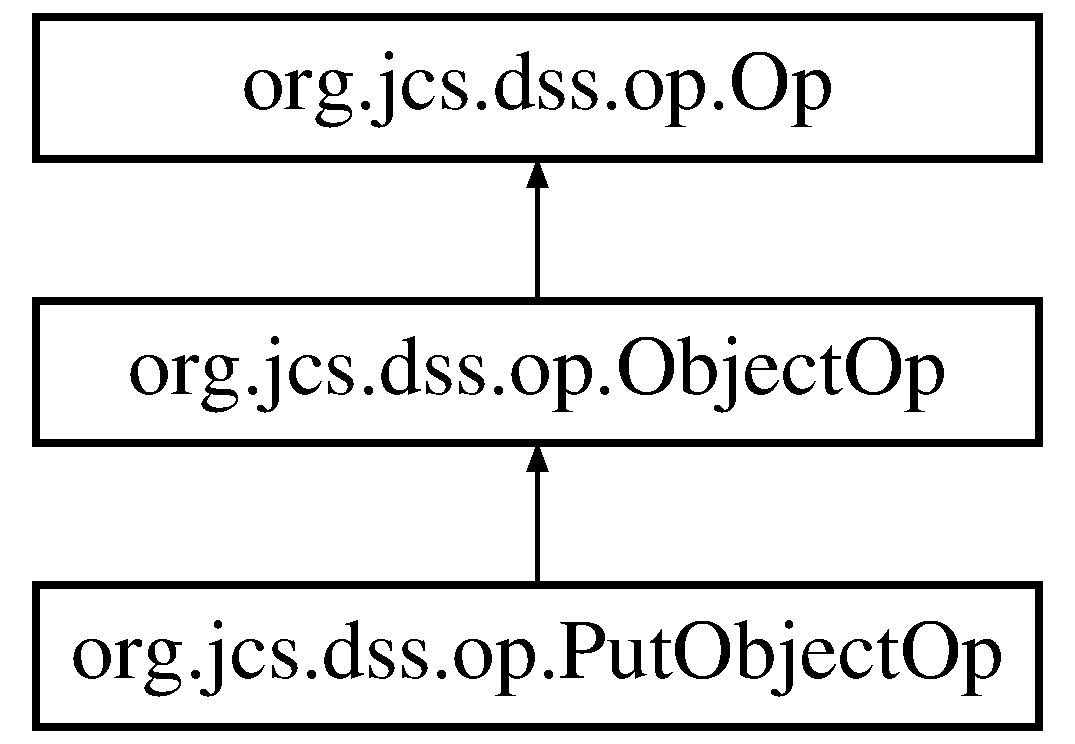
\includegraphics[height=3.000000cm]{classorg_1_1jcs_1_1dss_1_1op_1_1PutObjectOp}
\end{center}
\end{figure}
\subsection*{Public Member Functions}
\begin{DoxyCompactItemize}
\item 
\hyperlink{classorg_1_1jcs_1_1dss_1_1op_1_1PutObjectOp_abf3a9721db6ecb0329c028cb0bebdf8d}{Put\+Object\+Op} (Dss\+Connection conn, String bucket\+Name, String object\+Name, String filepath)  throws File\+Not\+Found\+Exception \hypertarget{classorg_1_1jcs_1_1dss_1_1op_1_1PutObjectOp_abf3a9721db6ecb0329c028cb0bebdf8d}{}\label{classorg_1_1jcs_1_1dss_1_1op_1_1PutObjectOp_abf3a9721db6ecb0329c028cb0bebdf8d}

\begin{DoxyCompactList}\small\item\em Constructors. \end{DoxyCompactList}\item 
Response \hyperlink{classorg_1_1jcs_1_1dss_1_1op_1_1PutObjectOp_a4858bcd90c98e27c0f123748b09bfee6}{execute} ()  throws Exception 
\begin{DoxyCompactList}\small\item\em Executes the method requested by user. \end{DoxyCompactList}\item 
Response \hyperlink{classorg_1_1jcs_1_1dss_1_1op_1_1PutObjectOp_a9f6ab4853d789ba25fe00c1a1a856d40}{make\+Request} ()  throws Exception 
\begin{DoxyCompactList}\small\item\em This method first gets signature, sets http\+Headers and then gets Response object. \end{DoxyCompactList}\item 
Object \hyperlink{classorg_1_1jcs_1_1dss_1_1op_1_1PutObjectOp_a54313a9bfbfe99696c87a5671771712d}{process\+Result} (Object resp)
\begin{DoxyCompactList}\small\item\em Method to extract E\+Tag and upload date of the uploaded object. \end{DoxyCompactList}\end{DoxyCompactItemize}
\subsection*{Additional Inherited Members}


\subsection{Detailed Description}
Class to Upload object file to the requested D\+SS bucket. 

\subsection{Member Function Documentation}
\index{org\+::jcs\+::dss\+::op\+::\+Put\+Object\+Op@{org\+::jcs\+::dss\+::op\+::\+Put\+Object\+Op}!execute@{execute}}
\index{execute@{execute}!org\+::jcs\+::dss\+::op\+::\+Put\+Object\+Op@{org\+::jcs\+::dss\+::op\+::\+Put\+Object\+Op}}
\subsubsection[{\texorpdfstring{execute()}{execute()}}]{\setlength{\rightskip}{0pt plus 5cm}Response org.\+jcs.\+dss.\+op.\+Put\+Object\+Op.\+execute (
\begin{DoxyParamCaption}
{}
\end{DoxyParamCaption}
) throws Exception\hspace{0.3cm}{\ttfamily [inline]}}\hypertarget{classorg_1_1jcs_1_1dss_1_1op_1_1PutObjectOp_a4858bcd90c98e27c0f123748b09bfee6}{}\label{classorg_1_1jcs_1_1dss_1_1op_1_1PutObjectOp_a4858bcd90c98e27c0f123748b09bfee6}


Executes the method requested by user. 

\begin{DoxyReturn}{Returns}
Response \+: Gets response object returned from \hyperlink{classorg_1_1jcs_1_1dss_1_1op_1_1PutObjectOp_a9f6ab4853d789ba25fe00c1a1a856d40}{make\+Request()} 
\end{DoxyReturn}

\begin{DoxyExceptions}{Exceptions}
{\em Exception} & \\
\hline
\end{DoxyExceptions}
\index{org\+::jcs\+::dss\+::op\+::\+Put\+Object\+Op@{org\+::jcs\+::dss\+::op\+::\+Put\+Object\+Op}!make\+Request@{make\+Request}}
\index{make\+Request@{make\+Request}!org\+::jcs\+::dss\+::op\+::\+Put\+Object\+Op@{org\+::jcs\+::dss\+::op\+::\+Put\+Object\+Op}}
\subsubsection[{\texorpdfstring{make\+Request()}{makeRequest()}}]{\setlength{\rightskip}{0pt plus 5cm}Response org.\+jcs.\+dss.\+op.\+Put\+Object\+Op.\+make\+Request (
\begin{DoxyParamCaption}
{}
\end{DoxyParamCaption}
) throws Exception\hspace{0.3cm}{\ttfamily [inline]}}\hypertarget{classorg_1_1jcs_1_1dss_1_1op_1_1PutObjectOp_a9f6ab4853d789ba25fe00c1a1a856d40}{}\label{classorg_1_1jcs_1_1dss_1_1op_1_1PutObjectOp_a9f6ab4853d789ba25fe00c1a1a856d40}


This method first gets signature, sets http\+Headers and then gets Response object. 

\begin{DoxyReturn}{Returns}
Response \+: response object by calling put method under Request class 
\end{DoxyReturn}

\begin{DoxyExceptions}{Exceptions}
{\em Exception} & \\
\hline
\end{DoxyExceptions}
Creating object of Dss\+Auth to get signature \index{org\+::jcs\+::dss\+::op\+::\+Put\+Object\+Op@{org\+::jcs\+::dss\+::op\+::\+Put\+Object\+Op}!process\+Result@{process\+Result}}
\index{process\+Result@{process\+Result}!org\+::jcs\+::dss\+::op\+::\+Put\+Object\+Op@{org\+::jcs\+::dss\+::op\+::\+Put\+Object\+Op}}
\subsubsection[{\texorpdfstring{process\+Result(\+Object resp)}{processResult(Object resp)}}]{\setlength{\rightskip}{0pt plus 5cm}Object org.\+jcs.\+dss.\+op.\+Put\+Object\+Op.\+process\+Result (
\begin{DoxyParamCaption}
\item[{Object}]{resp}
\end{DoxyParamCaption}
)\hspace{0.3cm}{\ttfamily [inline]}}\hypertarget{classorg_1_1jcs_1_1dss_1_1op_1_1PutObjectOp_a54313a9bfbfe99696c87a5671771712d}{}\label{classorg_1_1jcs_1_1dss_1_1op_1_1PutObjectOp_a54313a9bfbfe99696c87a5671771712d}


Method to extract E\+Tag and upload date of the uploaded object. 


\begin{DoxyParams}{Parameters}
{\em Response} & \+: response object by calling put method under Request class \\
\hline
\end{DoxyParams}
\begin{DoxyReturn}{Returns}
Put\+Object\+Result \+: Class containing E\+Tag and Upload date 
\end{DoxyReturn}


The documentation for this class was generated from the following file\+:\begin{DoxyCompactItemize}
\item 
Put\+Object\+Op.\+java\end{DoxyCompactItemize}

\hypertarget{classorg_1_1jcs_1_1dss_1_1op_1_1UploadPartOp}{}\section{org.\+jcs.\+dss.\+op.\+Upload\+Part\+Op Class Reference}
\label{classorg_1_1jcs_1_1dss_1_1op_1_1UploadPartOp}\index{org.\+jcs.\+dss.\+op.\+Upload\+Part\+Op@{org.\+jcs.\+dss.\+op.\+Upload\+Part\+Op}}


Class to execute Upload Part A\+PI.  


Inheritance diagram for org.\+jcs.\+dss.\+op.\+Upload\+Part\+Op\+:\begin{figure}[H]
\begin{center}
\leavevmode
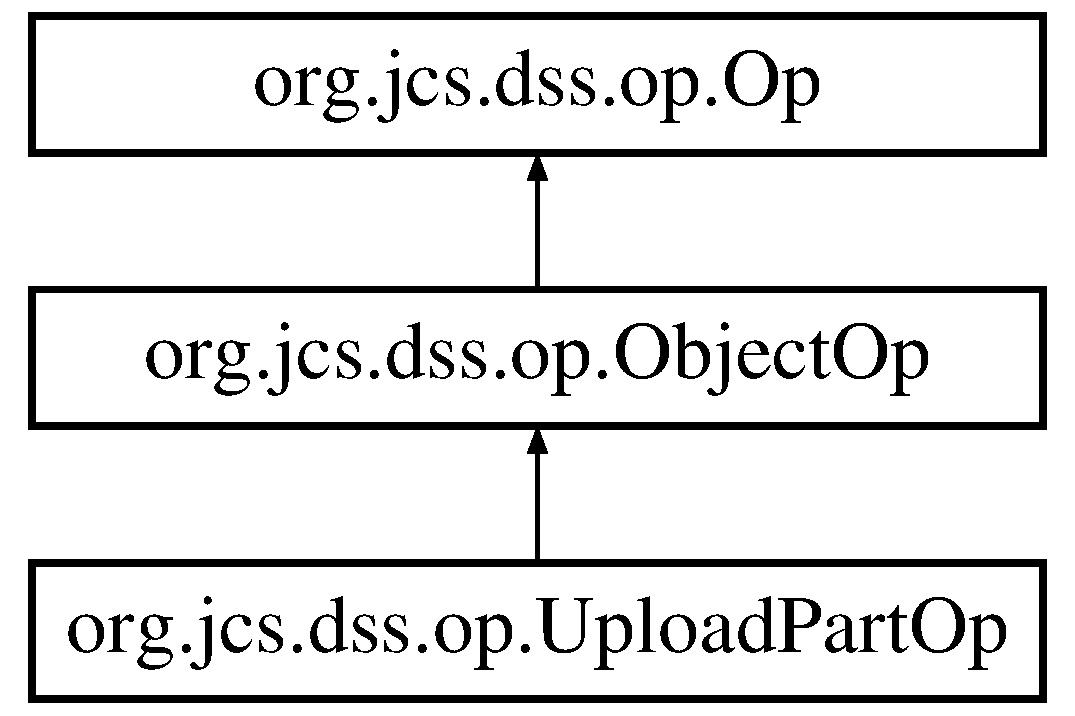
\includegraphics[height=3.000000cm]{classorg_1_1jcs_1_1dss_1_1op_1_1UploadPartOp}
\end{center}
\end{figure}
\subsection*{Public Member Functions}
\begin{DoxyCompactItemize}
\item 
\hyperlink{classorg_1_1jcs_1_1dss_1_1op_1_1UploadPartOp_a694f2d71544e9a9f899a3d07da6f0446}{Upload\+Part\+Op} (Dss\+Connection conn, String bucket\+Name, String object\+Name, String upload\+Id, String part\+Number, Input\+Stream in\+Stream)\hypertarget{classorg_1_1jcs_1_1dss_1_1op_1_1UploadPartOp_a694f2d71544e9a9f899a3d07da6f0446}{}\label{classorg_1_1jcs_1_1dss_1_1op_1_1UploadPartOp_a694f2d71544e9a9f899a3d07da6f0446}

\begin{DoxyCompactList}\small\item\em Constructors. \end{DoxyCompactList}\item 
Response \hyperlink{classorg_1_1jcs_1_1dss_1_1op_1_1UploadPartOp_a609e28843a72dba3a60e48cbf2ccbce8}{execute} ()  throws Exception 
\begin{DoxyCompactList}\small\item\em Executes the method requested by user. \end{DoxyCompactList}\item 
Response \hyperlink{classorg_1_1jcs_1_1dss_1_1op_1_1UploadPartOp_a21c2b882a81a728e29cbb0de230c6344}{make\+Request} ()  throws Exception 
\begin{DoxyCompactList}\small\item\em This method first gets signature, sets http\+Headers and then gets Response object. \end{DoxyCompactList}\end{DoxyCompactItemize}
\subsection*{Additional Inherited Members}


\subsection{Detailed Description}
Class to execute Upload Part A\+PI. 

\subsection{Member Function Documentation}
\index{org\+::jcs\+::dss\+::op\+::\+Upload\+Part\+Op@{org\+::jcs\+::dss\+::op\+::\+Upload\+Part\+Op}!execute@{execute}}
\index{execute@{execute}!org\+::jcs\+::dss\+::op\+::\+Upload\+Part\+Op@{org\+::jcs\+::dss\+::op\+::\+Upload\+Part\+Op}}
\subsubsection[{\texorpdfstring{execute()}{execute()}}]{\setlength{\rightskip}{0pt plus 5cm}Response org.\+jcs.\+dss.\+op.\+Upload\+Part\+Op.\+execute (
\begin{DoxyParamCaption}
{}
\end{DoxyParamCaption}
) throws Exception\hspace{0.3cm}{\ttfamily [inline]}}\hypertarget{classorg_1_1jcs_1_1dss_1_1op_1_1UploadPartOp_a609e28843a72dba3a60e48cbf2ccbce8}{}\label{classorg_1_1jcs_1_1dss_1_1op_1_1UploadPartOp_a609e28843a72dba3a60e48cbf2ccbce8}


Executes the method requested by user. 

\begin{DoxyReturn}{Returns}
Response \+: Gets response object returned from \hyperlink{classorg_1_1jcs_1_1dss_1_1op_1_1UploadPartOp_a21c2b882a81a728e29cbb0de230c6344}{make\+Request()} 
\end{DoxyReturn}

\begin{DoxyExceptions}{Exceptions}
{\em Exception} & \\
\hline
\end{DoxyExceptions}
\index{org\+::jcs\+::dss\+::op\+::\+Upload\+Part\+Op@{org\+::jcs\+::dss\+::op\+::\+Upload\+Part\+Op}!make\+Request@{make\+Request}}
\index{make\+Request@{make\+Request}!org\+::jcs\+::dss\+::op\+::\+Upload\+Part\+Op@{org\+::jcs\+::dss\+::op\+::\+Upload\+Part\+Op}}
\subsubsection[{\texorpdfstring{make\+Request()}{makeRequest()}}]{\setlength{\rightskip}{0pt plus 5cm}Response org.\+jcs.\+dss.\+op.\+Upload\+Part\+Op.\+make\+Request (
\begin{DoxyParamCaption}
{}
\end{DoxyParamCaption}
) throws Exception\hspace{0.3cm}{\ttfamily [inline]}}\hypertarget{classorg_1_1jcs_1_1dss_1_1op_1_1UploadPartOp_a21c2b882a81a728e29cbb0de230c6344}{}\label{classorg_1_1jcs_1_1dss_1_1op_1_1UploadPartOp_a21c2b882a81a728e29cbb0de230c6344}


This method first gets signature, sets http\+Headers and then gets Response object. 

\begin{DoxyReturn}{Returns}
Response \+: response object by calling put method under Request class 
\end{DoxyReturn}

\begin{DoxyExceptions}{Exceptions}
{\em Exception} & \\
\hline
\end{DoxyExceptions}
Creating object of Dss\+Auth to get signature 

The documentation for this class was generated from the following file\+:\begin{DoxyCompactItemize}
\item 
Upload\+Part\+Op.\+java\end{DoxyCompactItemize}

%--- End generated contents ---

% Index
\backmatter
\newpage
\phantomsection
\clearemptydoublepage
\addcontentsline{toc}{chapter}{Index}
\printindex

\end{document}
